%%%%%%%%%%%%%%%%%%%%%%%%%%%%%%%%%%%%%%%%%%%%%%%%%%%%%%%%%%%%%%%%%%%%%%%%%%%%%%%%%%%%%%%%%
% This is a LaTeX template for Bachelor or Master theses at ZHAW, in accordance with the 
% guidelines provided here:
% https://www.zhaw.ch/en/lsfm/study/studiweb/master-ls/masters-thesis/
%
%
% This template is based on previous works by:
% Steve Gunn (http://users.ecs.soton.ac.uk/srg/softwaretools/document/templates/)
% Sunil Patel (http://www.sunilpatel.co.uk/thesis-template/)
% Matteo Delucchi (https://github.com/matteodelucchi/ZHAW_thesis-template)
%
% University specific changes were made by:
% Matteo Delucchi
% Norman Juchler
% 
% Template license:
% CC BY-NC-SA 3.0 (http://creativecommons.org/licenses/by-nc-sa/3.0/)
%%%%%%%%%%%%%%%%%%%%%%%%%%%%%%%%%%%%%%%%%%%%%%%%%%%%%%%%%%%%%%%%%%%%%%%%%%%%%%%%%%%%%%%%%

%----------------------------------------------------------------------------------------
% DOCUMENT SPECIFICATION
%----------------------------------------------------------------------------------------
\documentclass[
    11pt,                      % Default font size
    %oneside,                  % One-side binding. Default: Two-side binding / alternating margins
    english,                   % Language. Use ngerman for German (Neue Rechtschreibung)
    singlespacing,             % Spacing option: singlespacing, onehalfspacing or doublespacing
    %nolistspacing,            % Set spacing in lists to single
    %draft,                    % Enable draft mode: no pictures, no links, overfull hboxes indicated
    liststotoc,               % Include list of figures/tables/etc in the table of contents
    %toctotoc,                 % Include the main table of contents to the table of contents
    parskip,                  % Add vertical space between paragraphs
    %nohyperref,               % Disable links in the entire document
    % helveticafont,             % Uncomment to use Helvetica font
    headsepline,               % Show a horizontal line under the header
    %chapterinoneline,         % Place the chapter title and chapter number on one line
    consistentlayout,          % Have the same layout for special chapters: 
                               % declaration, abstract and acknowledgements
]{MastersDoctoralThesis}

% Uncomment the following lines to only include a subset of chapters.
% This is useful for long documents, as typesetting takes a bit of time
%\includeonly{
%    Front/titlepage,
%    Front/imprint,
%    Front/abstract,
%    %Front/declaration,
%    %Front/acknowledgements,
%    %Front/symbols,
%    Chapters/Chapter1,
%    %Chapters/Chapter2
%    }


%----------------------------------------------------------------------------------------
% PREAMBLE: PACKAGES AND CONFIGURATIONS
%----------------------------------------------------------------------------------------
% !TEX root = main.tex

%----------------------------
%   Fonts and characters
%----------------------------

% Support for special characters
\usepackage[utf8]{inputenc}    % Specify input encoding
\usepackage[T1]{fontenc}       % Specify font encoding
\usepackage{amssymb}       % Specify font encoding

% Set main fonts
% Fonts catalogue: https://tug.org/FontCatalogue/
\usepackage{mathpazo}          % Use the Palatino font by default
\usepackage{beramono}          % Override the monospace/typewriter font
\usepackage{caption}
\usepackage{subcaption}
\usepackage{multirow}
% ZHAW title font
% Try to load Helvetica Rounded Bold, and OpenType font.
% Loading OTF or system fonts is possible with XeLaTeX.
% If the document is compiled using pdfLaTeX, resort 
\usepackage{ifxetex}
\ifxetex
    \usepackage{fontspec}
    \newfontfamily\zhawtitlefont{Helvetica Rounded Bold}
\else
    \newcommand{\zhawtitlefont}{\scshape}
\fi

%\usepackage[scaled]{helvet}

%----------------------------
%   Environments
%----------------------------

\usepackage{caption}           % Customized caption
\usepackage{subcaption}        % Subfigure captions
\usepackage{makecell}          % Per-cell formatting in tables (\makecell)
\usepackage{pdfpages}          % Required to include PDF files/graphics (\includepdf)

\usepackage{todonotes}         % Introduces the command \todo
\setlength{\marginparwidth}{2.5cm} % Adjust this if the todo notes are out of margins

% Create boxes as follows:
% \begin{colorbox}{red}{2}
\usepackage{tcolorbox}
\newtcolorbox{textbox}[2]{
    arc=3pt,
    boxrule=#2pt,
    colback=#1!25!white,
    width=\textwidth,
    halign=left,
    valign=center,
    colframe=#1!75!black
}

%----------------------------
%   Colors
%----------------------------

% Set up colors
\usepackage{xcolor}
% ZHAW Blue: Pantone 2945 U / R0 G100 B166
\definecolor{zhawblue}{rgb}{0.00, 0.39, 0.65}
% Colors related to code listings
\definecolor{codegreen}{rgb}{0,0.6,0}
\definecolor{codegray}{rgb}{0.5,0.5,0.5}
\definecolor{codepurple}{rgb}{0.58,0,0.82}
\definecolor{codebackground}{rgb}{0.93,0.94,0.95}

%----------------------------
%   Code listings
%----------------------------

% Setup code listings
\usepackage{listings}
\lstdefinestyle{mystyle}{
    backgroundcolor=\color{codebackground},   
    commentstyle=\color{codegreen},
    keywordstyle=\color{magenta},
    numberstyle=\tiny\color{codegray},
    stringstyle=\color{codepurple},
    basicstyle=\ttfamily\footnotesize,
    breakatwhitespace=false,
    breaklines=true,
%    captionpos=b,
    keepspaces=true,
    numbers=left,
    numbersep=5pt,
    showspaces=false,
    showstringspaces=false,
    showtabs=false,
    tabsize=4
}
\lstset{style=mystyle}

% minted is an alternative code listing package. (See chapter 2)
% For it to run successfully, ensure the following:
% - the Python package Pygments. Install with the following command:
%       python -m pip install Pygments
% - pdflatex (or xelatex) is executed with the flag --shell-escape
%   If you are using a TEX editor, you can modify the typesetting 
%   command somewhere in the settings.
%\usepackage[outputdir=build]{minted}
%\usemintedstyle{xcode}
% For fancier coloring schemes, see here:
% https://tex.stackexchange.com/questions/585582
% One could also create an own style in Pygments
% https://pygments.org/docs/styles/#creating-own-styles

%----------------------------
%   References
%----------------------------

% Set up references
\usepackage[
    backend=biber,             % Use biber backend (an external tool)
    sorting=none,              % Enumerates the reference in order of their appearance
    style=numeric-comp         % Choose here your preferred citation style
]{biblatex}
\addbibresource{references.bib}   % The filename of the bibliography
\usepackage[autostyle=true]{csquotes} 
                               % Required to generate language-dependent quotes 
                               % in the bibliography

%----------------------------------------------------------------------------------------
%   MARGIN SETTINGS
%----------------------------------------------------------------------------------------

\geometry{
    paper=a4paper,      % Change to letterpaper for US letter
    inner=2.5cm,        % Inner margin
    outer=3.8cm,        % Outer margin
    top=1.5cm,          % Top margin
    bottom=1.5cm,       % Bottom margin
    bindingoffset=.5cm, % Binding offset
    %showframe,         % Show the type block of the page
}
\setlength{\parskip}{1em}
\usepackage{enumitem}          % Layout control for list environments (e.g, itemize)
%\setlist{noitemsep}           % Suppress extra spaces between items
%\setlist{nosep}               % Suppress spaces before/after list environments



%----------------------------------------------------------------------------------------
% THESIS INFORMATION: MODIFY THIS SECTION!
%----------------------------------------------------------------------------------------

% The information below is used in the following parts:
% - Title page
% - Imprint
% - Abstract / Zusammenfassung
% - Meta information of PDF

\thesistitle{Deep learning assisted X-ray photoelectron spectroscopy analysis}             % Thesis title,              command: \ttitle
\thesistype{Master Thesis}             % Type of thesis (e.g. Master Thesis) \ttype
\thesisdate{\today}                     % Date of submission                  \tdate
\keywords{XPS, x-ray, spectroscopy, photoelectron, deep learning}
                                        % Keywords for the thesis,            \keywordnames
\author{Kilian Koch}                  % Your name,                          \authorname
\degree{Master of Science ZFH}          % Degree name,                        \degreename
\studyprogram{Applied Computational Life Sciences, M.Sc.} 
                                        % Study program                       \studyprog
\studyprogramlink{https://www.zhaw.ch/en/lsfm/study/master/applied-computational-life-sciences/}
                                        % Link to study program               \studyproglink

\supervisorA{Dr. Martin Schüle}       % Name of supervisor 1,               \supnameA
\supervisorAmail{martin.schuele@zhaw.ch}         % Email address of supervisor 1,      \supmailA
\supervisorAweb{https://www.zhaw.ch/de/ueber-uns/person/scli/}  %            \supwebA
\supervisorAinfo{                       % Formatted info about supervisor 1:  \supinfoA
    \supnameA\\
    Zurich University of Applied Sciences\\
    Email: \href{mailto:\supmailA}{\supmailA}\\
    Web: \href{\supwebA}{Link}
}

% Keep empty if there is no supervisor 2: \supervisorB{}
\supervisorB{PD Dr. Andreas Borgschulte}              % Name of supervisor 2,               \supnameB
\supervisorBmail{andreas.borgschulte@empa.ch}       % Email address of supervisor 2,      \supmailB
\supervisorBweb{https://www.empa.ch/web/s502/research}                  % \supwebB
\supervisorBinfo{                       % Formatted info about supervisor 2:  \supinfoB
    \supnameB\\
    University of Zurich\\
    Email: \href{mailto:\supmailB}{\supmailB}\\
    Web: \href{\supwebB}{Link}
}

\university{Zurich University of Applied Sciences}
                                        % University name                     \univname
\universitygerman{Zürcher Hochschule für Angewandte Wissenschaften}
                                        % University, in German               \univnameger
\department{Life Sciences and Facility Management} 
                                        % Department,                         \deptname
\institute{Institute of Computational Life Sciences} 
                                        % Institute,                          \instname
\group{Center of Computational Health} 
                                        % Research group                      \groupname

% Links
\universitylink      {https://www.zhaw.ch/en/university/}                   % \univlink
\universitylinkgerman{https://www.zhaw.ch/de/university/}                   % \univlinkger
\departmentlink      {https://www.zhaw.ch/de/lsfm/}                         % \deptlink
\institutelink       {https://www.zhaw.ch/en/lsfm/institutes-centres/icls/} % \instlink
\grouplink           {https://www.zhaw.ch/en/lsfm/institutes-centres/icls/computational-health/} % \grplink



\AtBeginDocument{
\hypersetup{pdftitle=\ttitle} % Set the PDF's title to your title
\hypersetup{pdfauthor=\authorname} % Set the PDF's author to your name
\hypersetup{pdfkeywords=\keywordnames} % Set the PDF's keywords to your keywords
}

\begin{document}
\frontmatter                  % Roman page numbering for the pre-content pages
\pagestyle{plain}             % Default to the plain heading style until the thesis style 
                              % is called for the body content


%----------------------------------------------------------------------------------------
% TITLE PAGE AND IMPRINT
%----------------------------------------------------------------------------------------
\include{Front/titlepage}
\let\cleardoublepage\clearpage
\include{Front/imprint}


%----------------------------------------------------------------------------------------
% DECLARATION
%----------------------------------------------------------------------------------------
% Comment out this section if the declaration of originality from ZHAW is used.
%% !TEX root = ../main.tex

%----------------------------------------------------------------------------------------
% APPENDIX: DECLARATION OF ORIGINALITY
%----------------------------------------------------------------------------------------

% Include the official "Plagiatserklärung" as a PDF

% Ensure that a TOC entry is create while suppressing the chapter header
\cleardoublepage
\phantomsection
\addtocounter{chapter}{1}
\addcontentsline{toc}{chapter}{\protect\numberline{\thechapter} Declaration of Originality}
% The above replaces this command (which creates a chapter header).
%\chapter{Declaration of Originality} % Main appendix title
\label{DeclarationOfOriginalityZHAW}

% Include a PDF (full page)

\includepdf[pages=-]{Appendices/Declaration of originality Master's Thesis.pdf}

\cleardoublepage


%----------------------------------------------------------------------------------------
% ABSTRACT
%----------------------------------------------------------------------------------------
% !TEX root = ../main.tex

%----------------------------------------------------------------------------------------
% ABSTRACT PAGE
%----------------------------------------------------------------------------------------
\begin{abstract}
\addchaptertocentry{\abstractname} % Add the abstract to the table of contents
Surface analysis for the determination of chemical composition of a solid palys an important role in material sciences. X-ray photoelectron spectroscopy is widely applied for such structural analysis, giving information beyond the outermost surface, as it probes deeper to approximately 10 nanometers depth. Analysis of the spectrum to model the solid under investigation is complex, as many effects complain the inference, such as inelastic and elastic scattering and sample contamination. This work applies deep learning models to three main problems; qualitative identification, quantitative identification and depth profiling.
To overcome the lack of available labelled XPS data, a simulation software was used to obtain >300k XPS spectra as training data. Four different models architectures were applied to the main problems; convolutional neural network (CNN), convolutional dct-informed neural network (CNN-DCT), Residual convolutional block attention model (CBAM) and Vision Transformer (ViT). 
\end{abstract}


%----------------------------------------------------------------------------------------
% German ABSTRACT PAGE
%----------------------------------------------------------------------------------------
\begin{extraAbstract}
\addchaptertocentry{\extraabstractname} % Add the abstract to the table of contents

Die Zusammenfassung entspricht einer Miniaturversion des gesamten Dokuments. Gliedere sie ähnlich: Beginne mit dem Kontext und der Motivation für das Projekt, einer kurzen Beschreibung der Methode und der verfügbaren Daten, Ihren Ergebnissen und den Schlussfolgerungen. Beschränke dich auf eine Seite!    
\end{extraAbstract}



%----------------------------------------------------------------------------------------
% ACKNOWLEDGEMENTS
%----------------------------------------------------------------------------------------
%\include{Front/acknowledgements}


%----------------------------------------------------------------------------------------
% LIST OF CONTENTS/FIGURES/TABLES PAGES
%----------------------------------------------------------------------------------------
% Comment out if any of the following is not needed:
\tableofcontents  % Add main table of contents
%\listoffigures    % Add list of figures
%\listoftables     % Add list of tables


%----------------------------------------------------------------------------------------
% ABBREVIATIONS / SYMBOLS
%----------------------------------------------------------------------------------------
%\include{Front/symbols}


%----------------------------------------------------------------------------------------
% DEDICATION
%----------------------------------------------------------------------------------------
\dedicatory{For/Dedicated to/To my\ldots} 


%----------------------------------------------------------------------------------------
% THESIS CONTENT - CHAPTERS
%----------------------------------------------------------------------------------------
\mainmatter % Begin numeric (1,2,3...) page numbering
\pagestyle{thesis} % Return the page headers back to the "thesis" style

% Include the chapters of the thesis as separate files from the Chapters folder
% Uncomment the lines as you write the chapters

% Indicate the main file. Must go at the beginning of the file.
% !TEX root = ../main.tex

%----------------------------------------------------------------------------------------
% CHAPTER 1
%----------------------------------------------------------------------------------------



\chapter{Introduction} % Main chapter title
\label{Chapter1} % For referencing the chapter elsewhere, use \ref{Chapter1} 

%----------------------------------------------------------------------------------------

% Define some commands to keep the formatting separated from the content
% Placing such commands in the preamble is a good idea.
\newcommand{\keyword}[1]{\textbf{#1}}
\newcommand{\tabhead}[1]{\textbf{#1}}
\newcommand{\code}[1]{\texttt{#1}}
\newcommand{\file}[1]{\texttt{\bfseries#1}}
\newcommand{\option}[1]{\texttt{\itshape#1}}

%----------------------------------------------------------------------------------------



%----------------------------------------------------------------------------------------

\section{X-ray photoelectron spectroscopy}


\subsection{Files}

Included are also several files, most of them are plain text and you can see their contents in a text editor. After initial compilation, you will see that more auxiliary files are created by \LaTeX{} or BibTeX and which you don't need to delete or worry about:

\keyword{example.bib} -- this is an important file that contains all the bibliographic information and references that you will be citing in the thesis for use with BibTeX. You can write it manually, but there are reference manager programs available that will create and manage it for you. Bibliographies in \LaTeX{} are a large subject and you may need to read about BibTeX before starting with this. Many modern reference managers will allow you to export your references in BibTeX format which greatly eases the amount of work you have to do.

\keyword{MastersDoctoralThesis.cls} -- this is an important file. It is the class file that tells \LaTeX{} how to format the thesis. 

\keyword{main.pdf} -- this is your beautifully typeset thesis (in the PDF file format) created by \LaTeX{}. It is supplied in the PDF with the template and after you compile the template you should get an identical version.

\keyword{main.tex} -- this is an important file. This is the file that you tell \LaTeX{} to compile to produce your thesis as a PDF file. It contains the framework and constructs that tell \LaTeX{} how to layout the thesis. It is heavily commented so you can read exactly what each line of code does and why it is there. After you put your own information into the \emph{THESIS INFORMATION} block -- you have now started your thesis!


%----------------------------------------------------------------------------------------

\section{Filling in Your Information in the \file{main.tex} File}\label{FillingFile}

You will need to personalise the thesis template and make it your own by filling in your own information. This is done by editing the \file{main.tex} file in a text editor or your favourite LaTeX environment.

Open the file and scroll down to the third large block titled \emph{THESIS INFORMATION} where you can see the entries for \emph{University Name}, \emph{Department Name}, etc \ldots

Fill out the information about yourself, your group and institution. You can also insert web links, if you do, make sure you use the full URL, including the \code{http://} for this. If you don't want these to be linked, simply remove the \verb|\href{url}{name}| and only leave the name.

When you have done this, save the file and recompile \code{main.tex}. All the information you filled in should now be in the PDF, complete with web links. You can now begin your thesis proper!

%----------------------------------------------------------------------------------------

\section{The \code{main.tex} File Explained}

The \file{main.tex} file contains the structure of the thesis. There are plenty of written comments that explain what pages, sections and formatting the \LaTeX{} code is creating. Each major document element is divided into commented blocks with titles in all capitals to make it obvious what the following bit of code is doing. Initially there seems to be a lot of \LaTeX{} code, but this is all formatting, and it has all been taken care of so you don't have to do it.

Begin by checking that your information on the title page is correct. For the thesis declaration, your institution may insist on something different than the text given. If this is the case, just replace what you see with what is required in the \emph{DECLARATION PAGE} block.

Then comes a page which contains a funny quote. You can put your own, or quote your favourite scientist, author, person, and so on. Make sure to put the name of the person who you took the quote from.

Following this is the abstract page which summarises your work in a condensed way and can almost be used as a standalone document to describe what you have done. The text you write will cause the heading to move up so don't worry about running out of space.

Next come the acknowledgements. On this page, write about all the people who you wish to thank (not forgetting parents, partners and your advisor/supervisor).

The contents pages, list of figures and tables are all taken care of for you and do not need to be manually created or edited. The next set of pages are more likely to be optional and can be deleted since they are for a more technical thesis: insert a list of abbreviations you have used in the thesis, then a list of the physical constants and numbers you refer to and finally, a list of mathematical symbols used in any formulae. Making the effort to fill these tables means the reader has a one-stop place to refer to instead of searching the internet and references to try and find out what you meant by certain abbreviations or symbols.

The list of symbols is split into the Roman and Greek alphabets. Whereas the abbreviations and symbols ought to be listed in alphabetical order (and this is \emph{not} done automatically for you) the list of physical constants should be grouped into similar themes.

The next page contains a one line dedication. Who will you dedicate your thesis to?

Finally, there is the block where the chapters are included. Uncomment the lines (delete the \code{\%} character) as you write the chapters. Each chapter should be written in its own file and put into the \emph{Chapters} folder and named \file{Chapter1}, \file{Chapter2}, etc\ldots Similarly for the appendices, uncomment the lines as you need them. Each appendix should go into its own file and placed in the \emph{Appendices} folder.

After the preamble, chapters and appendices finally comes the bibliography. The bibliography style (called \option{authoryear}) is used for the bibliography and is a fully featured style that will even include links to where the referenced paper can be found online. Do not underestimate how grateful your reader will be to find that a reference to a paper is just a click away. Of course, this relies on you putting the URL information into the BibTeX file in the first place.

%----------------------------------------------------------------------------------------

\section{Thesis Features and Conventions}\label{ThesisConventions}

To get the best out of this template, there are a few conventions that you may want to follow.

One of the most important (and most difficult) things to keep track of in such a long document as a thesis is consistency. Using certain conventions and ways of doing things (such as using a Todo list) makes the job easier. Of course, all of these are optional and you can adopt your own method.

\subsection{Printing Format}

This thesis template is designed for double sided printing (i.e. content on the front and back of pages) as most theses are printed and bound this way. To switch to one sided printing, uncomment the \option{oneside} option of the \code{documentclass} command at the top of the \file{main.tex} file. You may then wish to adjust the margins to suit specifications from your institution.

The headers for the pages contain the page number on the outer side (so it is easy to flick through to the page you want) and the chapter name on the inner side.

The text is set to 11 point by default with single line spacing, again, you can tune the text size and spacing should you want or need to using the options at the very start of \file{main.tex}. The spacing can be changed similarly by replacing the \option{singlespacing} with \option{onehalfspacing} or \option{doublespacing}.

\subsection{Using US Letter Paper}

The paper size used in the template is A4, which is the standard size in Europe. If you are using this thesis template elsewhere and particularly in the United States, then you may have to change the A4 paper size to the US Letter size. This can be done in the margins settings section in \file{main.tex}.

Due to the differences in the paper size, the resulting margins may be different to what you like or require (as it is common for institutions to dictate certain margin sizes). If this is the case, then the margin sizes can be tweaked by modifying the values in the same block as where you set the paper size. Now your document should be set up for US Letter paper size with suitable margins.

\subsection{References}

The \code{biblatex} package is used to format the bibliography and inserts references such as this one \parencite{Reference1}. 
The inline citation style can be changed to e.g. authoryear in the \file{main.tex} file. 
\href{https://www.overleaf.com/learn/latex/Biblatex_citation_styles}{This documentation} lists and explains different standard citation styles.
The options used in the \file{main.tex} file mean that the in-text citations of references are formatted with the author(s) listed with the date of the publication. Multiple references are separated by semicolons (e.g. \parencite{Reference2, Reference1}) and references with more than three authors only show the first author with \emph{et al.} indicating there are more authors (e.g. \parencite{Reference3}). This is done automatically for you. To see how you use references, have a look at the \file{Chapter1.tex} source file. Many reference managers allow you to simply drag the reference into the document as you type.

Scientific references should come \emph{before} the punctuation mark if there is one (such as a comma or period). The same goes for footnotes\footnote{Such as this footnote, here down at the bottom of the page.}. You can change this but the most important thing is to keep the convention consistent throughout the thesis. Footnotes themselves should be full, descriptive sentences (beginning with a capital letter and ending with a full stop). The APA6 states: \enquote{Footnote numbers should be superscripted, [...], following any punctuation mark except a dash.} The Chicago manual of style states: \enquote{A note number should be placed at the end of a sentence or clause. The number follows any punctuation mark except the dash, which it precedes. It follows a closing parenthesis.}

The bibliography is typeset with references listed in alphabetical order by the first author's last name. This is similar to the APA referencing style. To see how \LaTeX{} typesets the bibliography, have a look at the very end of this document (or just click on the reference number links in in-text citations).

\subsubsection{A Note on bibtex}

The bibtex backend used in the template by default does not correctly handle unicode character encoding (i.e. "international" characters). You may see a warning about this in the compilation log and, if your references contain unicode characters, they may not show up correctly or at all. The solution to this is to use the biber backend instead of the outdated bibtex backend. This is done by finding this in \file{main.tex}: \option{backend=bibtex} and changing it to \option{backend=biber}. You will then need to delete all auxiliary BibTeX files and navigate to the template directory in your terminal (command prompt). Once there, simply type \code{biber main} and biber will compile your bibliography. You can then compile \file{main.tex} as normal and your bibliography will be updated. An alternative is to set up your LaTeX editor to compile with biber instead of bibtex, see \href{http://tex.stackexchange.com/questions/154751/biblatex-with-biber-configuring-my-editor-to-avoid-undefined-citations/}{here} for how to do this for various editors.

\subsection{Tables}

Tables are an important way of displaying your results, below is an example table which was generated with this code:

{\small
    \begin{verbatim}
    \begin{table}
    \caption{The effects of treatments X and Y 
            on the four groups studied.}
    \label{tab:treatments}
    \centering
    \begin{tabular}{l l l}
    \toprule
    \tabhead{Groups} & \tabhead{Treatment X} & \tabhead{Treatment Y} \\
    \midrule
    1 & 0.2 & 0.8\\
    2 & 0.17 & 0.7\\
    3 & 0.24 & 0.75\\
    4 & 0.68 & 0.3\\
    \bottomrule\\
    \end{tabular}
    \end{table}
    \end{verbatim}
}

\begin{table}
\caption{The effects of treatments X and Y on the four groups studied.}
\label{tab:treatments}
\centering
\begin{tabular}{l l l}
\toprule
\tabhead{Groups} & \tabhead{Treatment X} & \tabhead{Treatment Y} \\
\midrule
1 & 0.2 & 0.8\\
2 & 0.17 & 0.7\\
3 & 0.24 & 0.75\\
4 & 0.68 & 0.3\\
\bottomrule\\
\end{tabular}
\end{table}

You can reference tables with \verb|\ref{<label>}| where the label is defined within the table environment. See \file{Chapter1.tex} for an example of the label and citation (e.g. Table~\ref{tab:treatments}).

\subsection{Figures}

There will hopefully be many figures in your thesis (that should be placed in the \emph{Figures} folder). The way to insert figures into your thesis is to use a code template like this:
\begin{verbatim}
\begin{figure}
\centering

\includegraphics{Figures/Electron}
\decoRule
\caption[An Electron]{An electron (artist's impression).}
\label{fig:Electron}
\end{figure}
\end{verbatim}
Also look in the source file. Putting this code into the source file produces the picture of the electron that you can see in the figure below.

\begin{figure}[th]
\centering

\includegraphics{Figures/Electron}
\decoRule
\caption[An Electron]{An electron (artist's impression).}
\label{fig:Electron}
\end{figure}

Sometimes figures don't always appear where you write them in the source. The placement depends on how much space there is on the page for the figure. Sometimes there is not enough room to fit a figure directly where it should go (in relation to the text) and so \LaTeX{} puts it at the top of the next page. Positioning figures is the job of \LaTeX{} and so you should only worry about making them look good!

Figures usually should have captions just in case you need to refer to them (such as in Figure~\ref{fig:Electron}). The \verb|\caption| command contains two parts, the first part, inside the square brackets is the title that will appear in the \emph{List of Figures}, and so should be short. The second part in the curly brackets should contain the longer and more descriptive caption text.

The \verb|\decoRule| command is optional and simply puts an aesthetic horizontal line below the image. If you do this for one image, do it for all of them.

\LaTeX{} is capable of using images in pdf, jpg and png format.

\subsection{Typesetting mathematics}

If your thesis is going to contain heavy mathematical content, be sure that \LaTeX{} will make it look beautiful, even though it won't be able to solve the equations for you.

The \enquote{Not So Short Introduction to \LaTeX} (available on \href{http://www.ctan.org/tex-archive/info/lshort/english/lshort.pdf}{CTAN}) should tell you everything you need to know for most cases of typesetting mathematics. If you need more information, a much more thorough mathematical guide is available from the AMS called, \enquote{A Short Math Guide to \LaTeX} and can be downloaded from:
\url{ftp://ftp.ams.org/pub/tex/doc/amsmath/short-math-guide.pdf}

There are many different \LaTeX{} symbols to remember, luckily you can find the most common symbols in \href{http://ctan.org/pkg/comprehensive}{The Comprehensive \LaTeX~Symbol List}.

You can write an equation, which is automatically given an equation number by \LaTeX{} like this:
\begin{verbatim}
\begin{equation}
E = mc^{2}
\label{eqn:Einstein}
\end{equation}
\end{verbatim}

This will produce Einstein's famous energy-matter equivalence equation:
\begin{equation}
E = mc^{2}
\label{eqn:Einstein}
\end{equation}

All equations you write (which are not in the middle of paragraph text) are automatically given equation numbers by \LaTeX{}. If you don't want a particular equation numbered, use the unnumbered form:
\begin{verbatim}
\[ a^{2}=4 \]
\end{verbatim}

%----------------------------------------------------------------------------------------

\section{Sectioning and Subsectioning}

You should break your thesis up into nice, bite-sized sections and subsections. \LaTeX{} automatically builds a table of contents by looking at all \verb|\chapter{}|, \verb|\section{}|  and \verb|\subsection{}| commands you write in the source.

The Table of Contents should only list the sections to three (3) levels. A \verb|chapter{}| is level zero (0). A \verb|\section{}| is level one (1) and so a \verb|\subsection{}| is level two (2). In your thesis it is likely that you will even use a \verb|subsubsection{}|, which is level three (3). The depth to which the Table of Contents is formatted is set within \file{MastersDoctoralThesis.cls}. If you need this changed, you can do it in \file{main.tex}.

%----------------------------------------------------------------------------------------

\section{In Closing}

You have reached the end of this mini-guide. You can now rename or overwrite this pdf file and begin writing your own \file{Chapter1.tex} and the rest of your thesis. The easy work of setting up the structure and framework has been taken care of for you. It's now your job to fill it out!

Good luck and have lots of fun!

\begin{flushright}
Guide written by ---\\
Sunil Patel: \href{http://www.sunilpatel.co.uk}{www.sunilpatel.co.uk}\\
Vel: \href{http://www.LaTeXTemplates.com}{LaTeXTemplates.com}
\end{flushright}

% Indicate the main file. Must go at the beginning of the file.
% !TEX root = ../main.tex

%----------------------------------------------------------------------------------------
% CHAPTER 2
%----------------------------------------------------------------------------------------

\chapter{Theory}

\label{Chapter2} % For referencing the chapter elsewhere, use \ref{Chapter2} 

%----------------------------------------------------------------------------------------
\label{XPS_theory}
\section{X-ray photoelectron spectroscopic analysis}
\subsection{Principle of measurement}
Photoelectron spectroscopy (PES) hinges on the fundamental principle of the photoelectric effect  as elucidated through the photon theory by Einstein and Rutherford \cite{rutherford_xxxvii_1914, einstein_uber_1905}. This concept essentially explains how incident light hitting a material results in the emission of electrons, known as photoelectrons.
In X-ray photoelectron spectroscopy, soft x-rays are commonly generated by exciting Aluminum or Manganese to radiate K \(\alpha\) x-rays with 1486.6 eV and 1253.6 eV respectively. These x-ray sources have a small natural linewidth and thus can provide high resolution. The produced photons then interact with the sample which in turn emit electrons, making use of the photoelectric effect previously described. Those electrons are then transported to a multichannel detector which counts the electrons. To improve, detector efficiency and electron collection, and thus the resolution, a monochromator is usually used.\cite{stevie_introduction_2020} The concept of the measurement can be expressed as shown in eq. 1:
\begin{equation}
    hv = BE + KE + \psi spec
\end{equation}
which can be re-arranged to express the binding energy as a function of known variables \cite{stevie_introduction_2020} as shown in eq. 2
\begin{equation}
    BE = hv- KE - \psi spec
\end{equation}

\begin{figure}
    \centering
    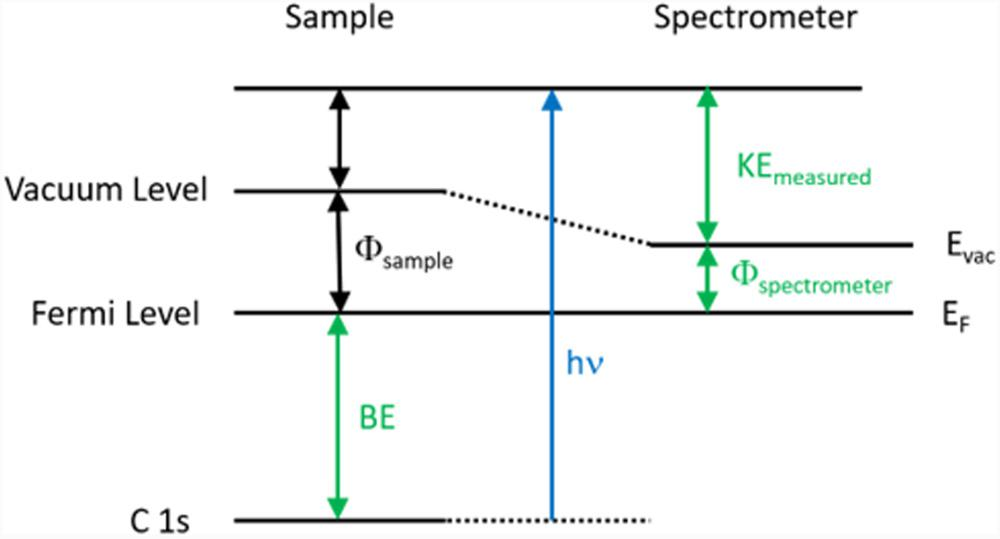
\includegraphics[width=0.7\textwidth]{Figures/image4_3.jpeg}
    \caption{The principle of measurement schematically illustrated}
    \label{fig:enter-label}
\end{figure}


The sample work function is a specific change in energy levels dependent on the chemical environment (coordination, charge etc.) of the atom of interest. It describes the work an electron must overcome to escape the local environment up to the vacuum level. 


The intensity of the peaks is indicated as counts and corresponds to the number of electrons that reach the detector during the acquisition time. Thus, the intensity of the signal depends on the acquisition time and should be normalized before comparing with spectra collected with unknown method and instrument parameters.
The complex and sample-specific interactions of the produced electrons with the sample are discussed in the next subchapter.

\subsection{Surface sensitivity}

The study of surface sensitivity in XPS has been thoroughly studied and summarized in multiple publications \cite{powell_surface_2009, }. Electrons emitted from the samples atoms can take different ways until they eventually reach the detector. They either take a direct path (A), are elastically scattered and return to the detector (B) or are inelastically scattered and do not return to the detector (C) as shown in Figure \ref{fig:scattering}.

To this point, there are three terms to describe surface sensitivity in XPS:
\begin{itemize}
\item The initial energy which is needed to overcome dielectric effects such that an electron can be lost from a material is described by the electron loss function (ELF)
\item Inelastic mean free path (IMFP), often denoted as $\lambda$, describes the distance an electron travels in a given material before inelastically scattering.
\item Effective attenuation length (EAL) is the length the electron travels into the sample while also considering elastic scattering effects.

\end{itemize}

\begin{figure}
    \centering
    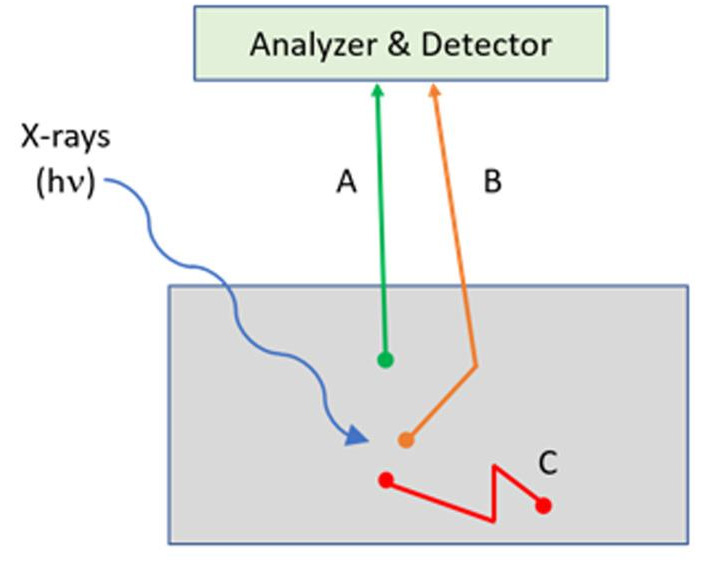
\includegraphics[width=0.3\textwidth]{Figures/image6_1.jpg}
    \caption{Scattering effects in XPS \cite{stevie_introduction_2020}}
    \label{fig:scattering}
\end{figure}

The intensity of electrons emmited from a sample deeper than $d$ can be described using Beer's law as shown in equation \ref{beerslaw}, where $I_{0}$ is the initial energy flux

\begin{equation}
\label{beerslaw}
    I = I_{0} * exp(-d/\lambda)
\end{equation}

Elastic electron scattering (see Figure \ref{fig:scattering} B), however, has often caused uncertainties in measurements of EAL and IMFP. The IMFP and the EAL are element specific and also depend on the kinetic energy. 
%As the IMFP does not consider elastic scattering, there is a universal curve describing overall tendencies. 
The information depth (ID) is often denoted as 3 $\lambda$, where statistically, 95\% of the information originates. From equation \ref{beerslaw}, it is obvious that the information obtained decays non-linearly, 

\subsection{X-ray photoelectron spectra} % identification?
\subsubsection{Direct transitions}
% Photoelectron peaks
As X-ray photoelectron spectroscopy uses x-rays to produce core-level electrons from a sample, the detection of these electrons is the desired origin of a so-called photoelectron peak, which originates in the photoionization effect. The notation for the photoelectron peaks is the element followed by the orbital from which they originate, such as C 1s for the Carbon peak from the 1s orbital \cite{stevie_introduction_2020}. In physical research, cross sections describe the probability of a certain process to take place when a certain material is subject to some radiant excitation. Thus, the photoionization cross section describes the probability of the photoionization process to happen. 

%satellite peaks 
While an electron is travelling towards the detector, it might interact with valence electrons of other atoms and lose some of its energy. This process is an energy-loss process and thus, the peak observed is shifted towards higher binding energy.

%multiplet splitting
A similar effect can be observed for unpaired electrons in the valence bands. The so-called multiplet splitting of photoelectron peaks is shown in Figure \ref{fig:peaks}.

%Multiplet splitting of core level peaks occurs when there are unpaired electrons in the valence levels and often results in unexpected peak splitting.


\subsubsection{Indirect transitions}
% Auger electron peaks, 
When a core electron is lost due to the X-ray excitation, a deficiency of electrons results. This ionized state is then relaxed with an electron from the outer-most so-called valence orbital \cite{stevie_introduction_2020}. This process induces the release of energy which can then be detected with XPS. It is crucial to note that this process is independent of the source energy and thus, the Auger peak binding energy changes when another source of X-rays is used. This is especially important to resolve issues when Auger peaks overlap with photoelectron peaks.


\begin{figure}[H]
    \centering
    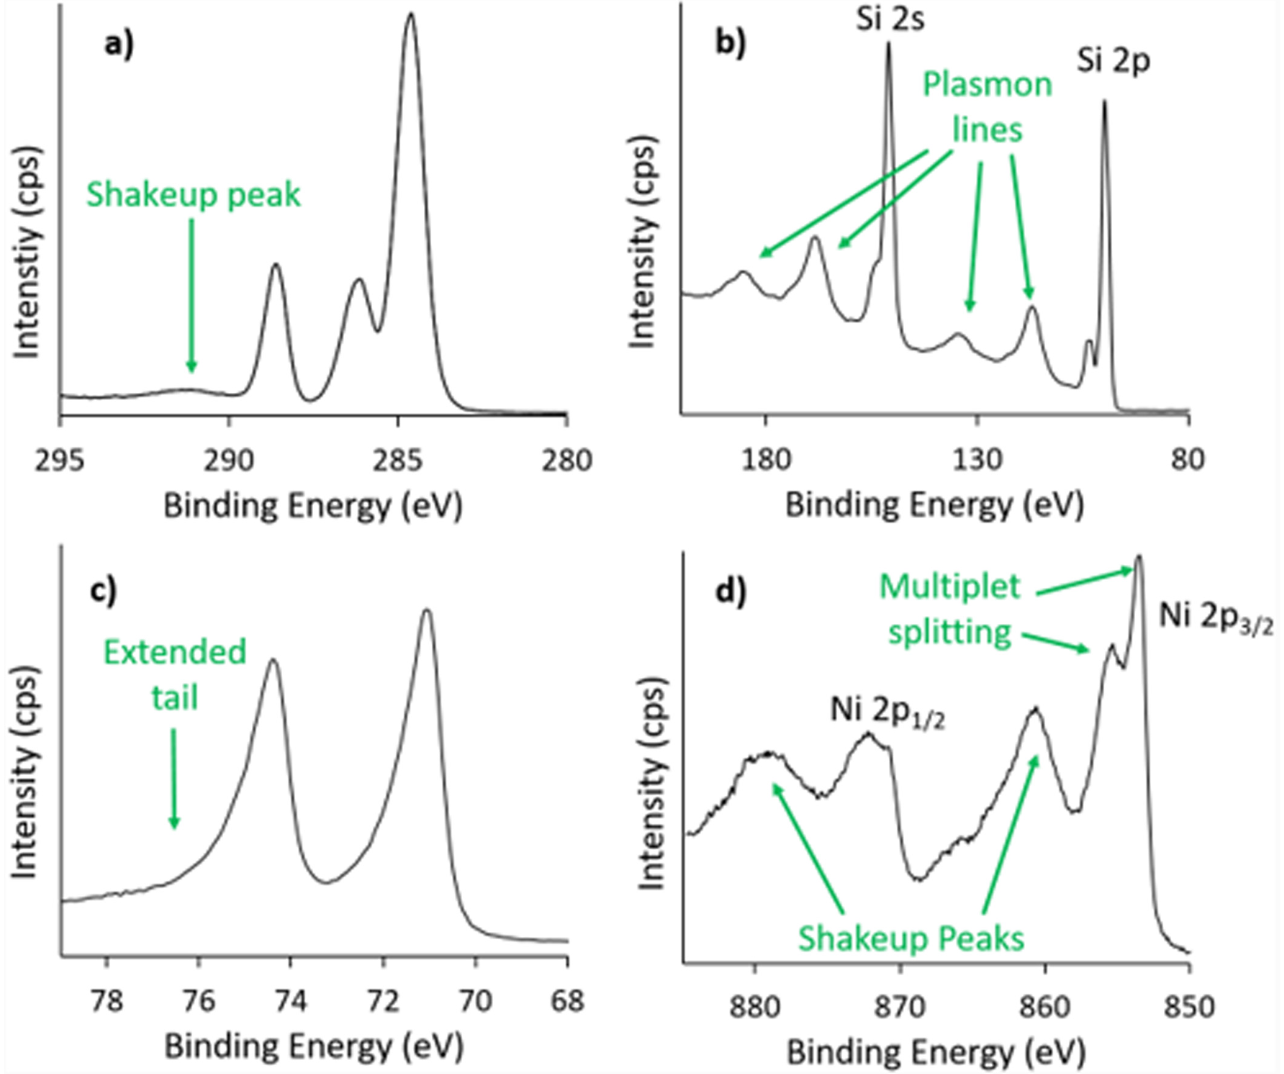
\includegraphics[width=0.75\textwidth]{Figures/peaks.png}
    \caption{Examples of peaks origin (a) C 1s spectrum of PET and its shakeup peak due to the shared $\pi$ electron system, (b) shakeup peaks due to the excitation of Silicon plasmon lines, (c) tailing on a metallic peak due to shakeup excitations (d) Ni 2p from \ch{NiO} - multiplet splitting and shakeup peaks \cite{stevie_introduction_2020}}
    \label{fig:peaks}
\end{figure}


% Plasmon peaks
Plasmon peaks are a special kind of shakeup peaks and arise from the excitation of plasmons. These so-called surface plasmons are formed when electrons from the substrate oscillate due to energy absorption and if the electrons produced by the X-ray source interact with the plasmon, losing kinetic energy. Mostly, this will occur in metals from the first and second group in the periodic table of elements due to the free electrons present that can form plasmons \cite{moulder_handbook_1992}.



\subsection{Adventitious Carbon}
    
When analyzing with XPS, we often find peaks which do not originate from the sample but from the atmosphere. As the atmosphere consists of organic compounds, they include O 1s and C 1s peaks. Often, the C 1s peak is used as a internal standard reference peak to shift the measured spectra to the correct position. This is done because peak shifts occur frequently owing to charging effects which arise from sample properties. Due to varying atmospheric composition, however, this peaks' position is uncertain and is itself  not clearly defined. \cite{biesinger_accessing_2022} As the peak reference to adventitious carbon is most frequently used, it should be considered when comparing, evaluating and analysing experimental data.
In addition, the contamination can be mostly removed when an ion-etching procedure is performed prior to the measurement. Although sometimes referred to as a \emph{contamination layer}, it does not behave similar to a layer, as it is not densely populated on the surface.

\subsection{Quantitative XPS Analysis}
As the quantity of a certain element increases, its corresponding peak should increase as well, given its generated electrons can still escape the sample without being scattered. However, simultaneously, other peaks decrease proportionally in intensity. For example, the peak area of \ch{Al2O3} should sum up to 2:3 for Al:O.
The common procedure for quantitative analysis is to substract the background according to a modelled assumption and subsequently elaborate a relative sensitivity factor (RSF) to measure the area under the peaks and set them into relation.

\subsection{Depth profiling}
In many areas of research, the investigation of surfaces, buried interfaces and quantification in relation to the sample depth is of interest. Experimentally, there exist four methods for investigating depth-information of a component in a sample. These are:
\begin{enumerate}
    \item Presence or absence of energy loss peaks which occur when electrons from deeper regions of the material need to travel to the surface and lose energy (associated to the elastic scattering effect)
    \item The intensity ratio of peaks across the kinetic energy (high vs low) – only suitable for a selection of elements (semi-qualitative).
    \item Controlled erosion and subsequent measurement of the surface (destructive and strong material dependency)
    \item Measurement at different sample-mounting angles (ARXPS). \cite{moulder_handbook_1992} 
    \end{enumerate}
and more recently have been extended by two additional methods:
\begin{enumerate}[resume]
    \item Combination with hard x-ray photoelectron spectroscopy (HAXPES) has become more accessible which in combination with XPS can give depth information of a sample \cite{zborowski_improved_2022}.
    \item Modelling of X-ray photoelectron spectra is another recent technique for the determination of depth distribution and has been investigated previously using manual approaches \cite{zborowski_comparison_2022}.

\end{enumerate}


Methods 1-3 have the drawback of being potentially destructive on the sample surface. Further, they are giving only very vague information about the samples’ depth profile; the accuracy is often denoted to be $\pm$10\%.
The non-destructive methods 4-6 (ARXPS / Modelling / XPS-HAXPES) are further explained, as they are comparable to the data-driven approach used in this work.

\subsubsection{Angle resolved XPS (ARXPS)}
\begin{figure}
    \centering
    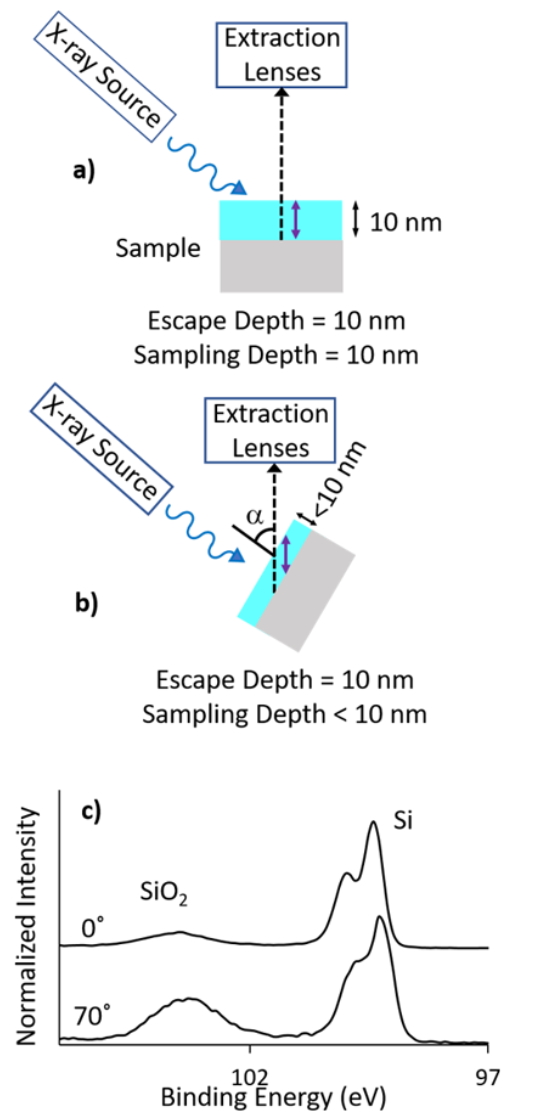
\includegraphics[width=0.4\textwidth]{Figures/ARXPS.png}
    \caption{Angle resolved XPS \cite{stevie_introduction_2020}}
    \label{fig:arxps}
\end{figure}
A variation on the XPS-technique involves measurements at different mounting-angles of the sample.
This changes the path the X-rays take into and out from the sample, as shown in Figure \ref{fig:arxps} which compares a standard 90\textdegree  take-off angle (a) with a smaller angle $\alpha$ (b). As the angle $\alpha$ decreases, the X-rays travel through a proportional higher amount of surface which in turn increases the sensitivity towards the surface. From the obtained spectra (c), we can deduct the thickness of the layers. This deduction is often done by Software which uses the Maximum entropy method first described by Smith et al. \cite{smith_maximum_1992} in 1992.
The intensity of the peaks in respect to the angle $\alpha$ is shown in equation \ref{intensity_angle}, where $G(\alpha)$ is a term representing geometric and instrumental factors and will cancel out as intensity ratios are considered. It should be noted that this assumes homogeneity of the two layers.
The thickness is denoted as $t$,
$\sigma$ is the photoelectron cross section,
F is the analyzer transmission function,
c is the atomic concentration,
z is the depth and $\lambda$ the IMFP or the EAL
\cite{paynter_arxps_2009}.

\begin{equation}
\label{intensity_angle}
    I_{t} = G(\alpha)\sigma F c \int_{0}^{t} e^{-z/ \lambda cos \alpha} dz
\end{equation}

A newer method collects spectra in parallel, thus is called pARXPS, which reduces acquisition time and constant transmission \cite{bure_assessing_2023}.

\subsubsection{XPS-HAXPES}

Hard X-ray photoelectoron spectroscopy is a technique similar to XPS, but uses Gallium or Chromium to produce hard x-rays to achieve much higher energy levels. As these X-rays are in the range of multiple keVs, the IMFP increases drastically and we are able to probe much deeper into the surface compared to XPS. Combining the two analyses can provide researchers with valuable information of the surface and the deeper regions of samples. This approach has been demonstrated to provide valuable information in multiple publications \cite{bure_assessing_2023, siol_concepts_2020} 

\subsection{Simulation with Sessa}
As XPS spectra are not available from databases in sufficient number for the use as training data in deep learning, we used the NIST Standard Reference Database 100 Software, also called Sessa \cite{noauthor_nist_2010, smekal_simulation_2005}. The development aimed to provide a solution to two main applications - quantitative XPS and simulation of layered samples. The proposed approach for layered systems and thickness analysis is to adjust the model "to find maximum consistency between simulated and measured spectra" \cite{smekal_simulation_2005}.
In Sessa, spectra are simulated using a Monte-Carlo method using the data provided from multiple databases for the following data:

\begin{itemize}
    \item elemental data
    \item differential inverse inelastic mean free path
    \item IMFP values
    \item differential elastic-scattering cross section
    \item total elastic-scattering cross section
    \item transport scattering cross section
    \item photoionization cross section
    \item photoionization asymmetry parameter
    \item electron inner-shell ionization cross section
    \item photoelectron lineshape
    \item binding energies of the elements.
\end{itemize}

Although the exact computational models used in Sessa are not public, Smekal et al. have shown that the linear approximation approach for the angle dependent cross sections, and the depth distribution function (which models surface sensitivity) are in good agreement with experimental data. However, they raise awareness to the need for empirical data in order to realistically model the shape of Auger peaks.

\label{DL_theory}
\section{Deep Learning for spectroscopic data}

Techniques of machine learning and deep learning specifically have been applied to spectroscopic data since the 1990s. It has been applied to a variety of spectroscopic methods such as Near Infrared Spectroscopy (NIR), Raman Spectroscopy, Nuclear Magnetic Resonance Spectroscopy (NMR) and Infrared Spectroscopy (IR) and Laser Induced Breakdown Spectroscopy (LIBS) \cite{krohling_1d_2023, sun_cnnlstm_2023, ma_conditional_2022, zhang_deep_2023, castorena_deep_2021, ghosh_deep_2019, huang_attention_2019}. However, chemometric or physics-based approaches have been and still are favored for data analysis due to the lack of model explainability for data-driven approaches. Because chemometrics is most often based on decomposition techniques such as Principal Component Analysis (PCA) and subsequent linear regression, it remains possible to interpret why a model predicts something by considering the loadings (weights) of the selected (principal) components. However, especially because of the non-linear learning capabilities of deep learning, they have been widely applied chemical analysis methods with complex underlying physical effects \cite{aires-de-sousa_prediction_2002}.

Deep learning has been previously applied to XPS-analysis by Drera et al.\cite{drera_deep_2019}. They achieved an overall performance of quantitative detection above 10$\%$ content, similar to the detection limit of users - they state. They used solely convolutional neural networks to build their prediction model. Their training data was constructed similarly to the data used in this work. Moreover, Hunt investigated depth profiling using XPS in combination with the singular value decomposition (SVD) algorithm \cite{hunt_depth_2000}. Additionally, Hunter modelled the impact of sample surface roughness on the prediction using the SVD algorithm and the Tyler regularization algorithm.

Attention-based neural networks have been applied to near infrared spectroscopy analysis of medical fungi \cite{huang_attention_2019} and sand gravel \cite{yuan_hybrid_2022} to successfully identify secondary parameters, such as moisture or polysaccharide content with similar or better results than the well-known partial least squares (PLS) fitting.

% advances in DL & applications to spectroscopy tasks

\subsection{Model hyperparameters \& training}
For each model, a set of hyperparameters define either initial, or fixed values used for the training. 

Multiple training cycles are performed on the dataset, which is shuffled before each training cycle, also called epoch. A so-called \emph{loss function} is introduced which in general resembles how far the predicted $\hat{y}$ labels are from the correct labels $y$ $(\hat{y} - y)$.
In each epoch, the weights of the model are re-evaluated subject to minimizing the defined loss-function with respect to the defined learning rate. The initial data available is split into a training and validation dataset. The weights are trained only the training dataset, while the validation dataset is used to check the performance on data which is new for the model and tune its hyperparameters. Model training is successful if we observe the training data loss decrease over the epochs. 


\subsection{General patterns}
\subsubsection{Loss functions and performance measures}
 A loss function generally computes how close the model predictions are to the labels, while the accuracy will describe what proportion of labels were predicted correctly. As the task can be of several types, such as regression, or classification, the loss and accuracy functions should be adapted accordingly. The functions used in this work will be explained hereafter.
The categorical crossentropy loss function is used for multi-class and multi-label classification problems. It is computed according to equation \ref{cce}, where $M$ is the number of classes, $y$ is the ground-truth and $p$ is the prediction of the observation $o$ of class $c$ \cite{noauthor_classical_nodate}. 
Categorical Accuracy computes the correctly predicted label based on the argmax function (the highest prediction value) of one-hot encoded labels.
\begin{equation}
\label{cce}
-\sum_{c=1}^My_{o,c}\log_{n}(p_{o,c})
\end{equation}

The binary crossentropy loss function is used for binary classification tasks, for example when we want to know whether a certain property is true or not. Similarly to the categorical crossentropy loss function, it computes the $log_{n}$ of the difference betweeen the true and the predicted values. In the binary case, we have $M=2$, so the function can be rewritten as $-{(y\log(p) + (1 - y)\log(1 - p))}$.


Binary accuracy

\subsection{General patterns}
\subsubsection{Loss functions and performance measures}
 A loss function generally computes how close the model predictions are to the labels, while the accuracy will describe what proportion of labels were predicted correctly. As the task can be of several types, such as regression, or classification, the loss and accuracy functions should be adapted accordingly. The functions used in this work will be explained hereafter.
The categorical crossentropy loss function is used for multi-class and multi-label classification problems. It is computed according to equation \ref{cce}, where $M$ is the number of classes, $y$ is the ground-truth and $p$ is the prediction of the observation $o$ of class $c$ \cite{noauthor_classical_nodate}. 
Categorical Accuracy computes the correctly predicted label based on the argmax function (the highest prediction value) of one-hot encoded labels.
\begin{equation}
\label{cce}
-\sum_{c=1}^My_{o,c}\log_{n}(p_{o,c})
\end{equation}

The binary crossentropy loss function is used for binary classification tasks, for example when we want to know whether a certain property is true or not. Similarly to the categorical crossentropy loss function, it computes the $log_{n}$ of the difference betweeen the true and the predicted values. In the binary case, we have $M=2$, so the function can be rewritten as $-{(y\log(p) + (1 - y)\log(1 - p))}$.
Binary accuracy
Mean Squared Error Loss
 
 
\subsubsection{Dense layers}
What is often referred to as fully connected, dense, feed-forward neural network or Multilayer Perceptron describes a network consisting of solely fully connected layers. These layers are connected in an $n:m$ manner, where each node of a layer with $n$ nodes is connected with each node of a layer with $m$ nodes. 

\subsubsection{Dropout}
Dropout layers are often used to regularize and generalize models. In these layers, which are fully connected layers, a certain percentage of nodes are not used during training and the specific unused nodes are selected from new each training cycle. This ensures that the training of the network does not rely on only a subset or even a single node, but on all nodes in a similar intensity. The fraction of nodes defined to drop each training cycle is denoted as $p$.

\subsubsection{Batch-Normalization}
Big datasets are usually divided into subsets such that we can efficiently train our network. This is done because the data might not fit the available computing memory and thus slow our computation. However, even if we randomly split the dataset, we will encounter a non-uniform distribution of information between our batches. Thus, in a batch-normalization layer, each batch input is normalized to have a mean of zero and a standard deviation of one. 
%The positive effects have been shown in multiple publications

\subsection{Convolutional Neural Networks (CNN)}
In convolutional neural networks (CNN), the input values are multiplied with a kernel to extract features. The CNNs are used where the input is of a discrete, grid-like topology. A kernel in this sense can represent a vector of n dimensions, where in case of spectra n=1 that will be moved along an axis, applying the multiplication subsequently. As the kernel can not be applied at the ends of our data, we can decide to apply padding on the ends with zero values, or start only when the kernel fits our data. Applying a kernel of size 5 on a vector of length 20 will thus only compute a vector of size 11 without padding, whereas its length will be 20 with the padding.
The values of the kernel are learnable, such that it can be fitted to extract specific features depending on the nature of the data.

These convolutional layers are usually followed by pooling layers - such as max-pooling or average-pooling - which also use a kernel. As the pooling layers reduce the dimensionality of the input, they have a number of positive effects on the model, such as better robustness to input variability and faster training. In addition, pooling layers help the model to learn invariances in the input data, such as rotation or small shift of an image content \cite{goodfellow_deep_2016}. 

The 1-dimensional convolutions we use in the case of spectral data will thus use $p$ one-dimensional kernels (vectors) of pre-defined length, where $p$ stands for the number of channels. If, for example, our spectrum vector is of length 1024, using a 1d-convolutional kernel of arbritary size with 16 channels will be applied. Thus, we will retain 16 vectors, each representing a feature of our spectrum. Arranging multiple CNN layers in sequence is a usual architecture used, as the layers learn from previously extracted features to represent more complex structures.

This network architectural pattern is extensively used in image classification tasks but has also been applied to diverse classification tasks, including spectroscopic data analysis \cite{sun_cnnlstm_2023, castorena_deep_2021, drera_deep_2019}.

\subsection{Residual networks (ResNet)}

In residual networks, the input is re-added after performing weighted operations such as convolutions. This feature has known positive effects, especially on deeper neural networks (networks with multiple layers). Residual network architectures diminish the well-known vanishing gradient problem by adding skip connections to the network. 

\begin{figure}[H]
    \centering
    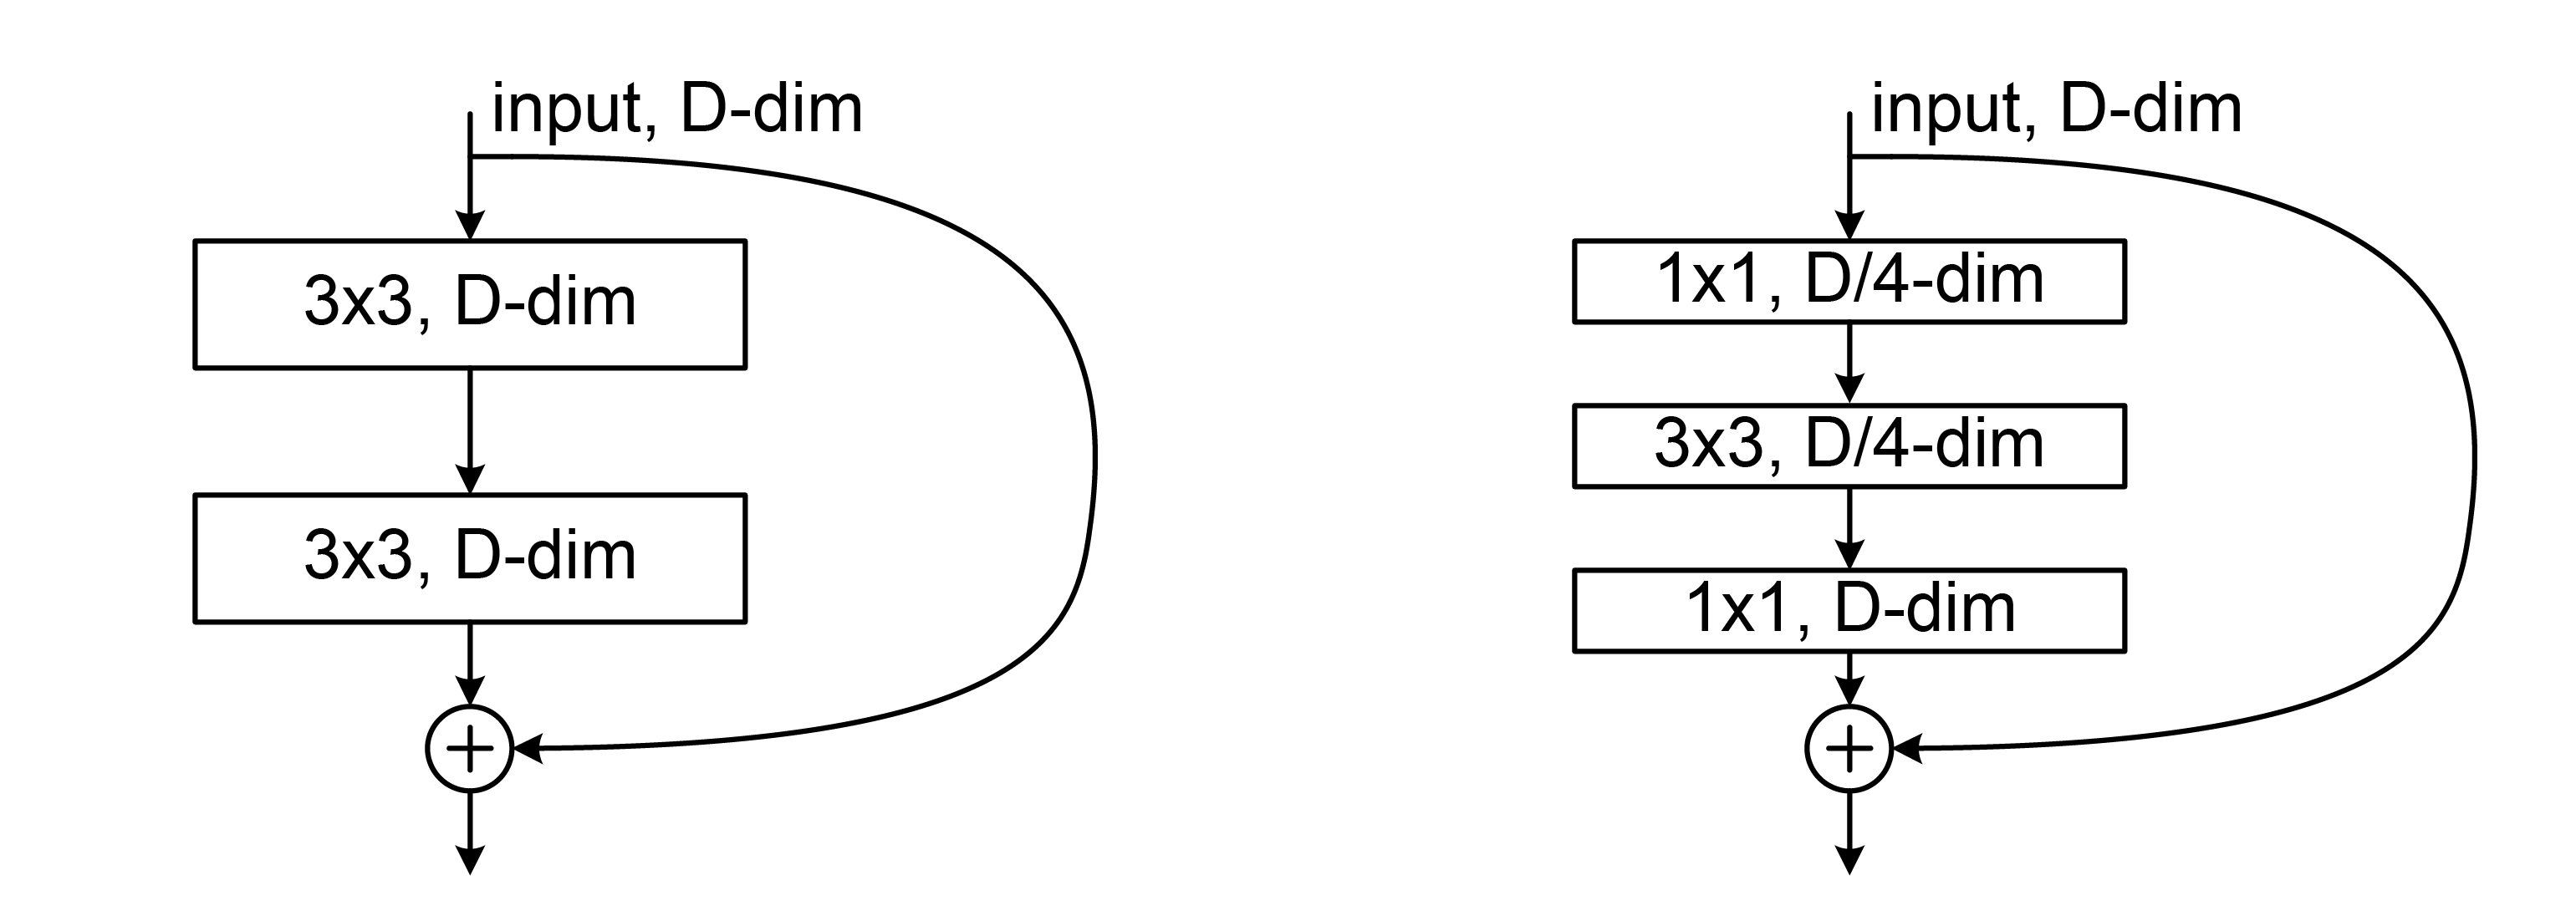
\includegraphics[width=0.5\textwidth]{Figures/ResBlockVariants.png}
    \caption{Residual block pattern}
    \label{fig:res_block}
\end{figure}

This pattern has later also been used for other models, as it allows much deeper networks to learn much more efficiently. Especially, in combination with convolutional models, this has improved the accuracy eg. in CBAM as explained below.

\subsection{Transformer-based networks}

Originally developed to solve neural language processing (NLP) tasks, the attention mechanism was first described in 2017 \cite{vaswani_attention_2023}.
The combination of an encoder-decoder paradigm with the Multi-Head Attention architecture lead to the development of the Transformer model. The most recent architecture used for NLP tasks is shown in Figure \ref{fig:transformer_model}.
A transformer consists of tokenizers, embedding layers and transformer layers which include the attention layers and multilayer perceptron (MLP) layers.

\begin{figure}[H]
    \centering
    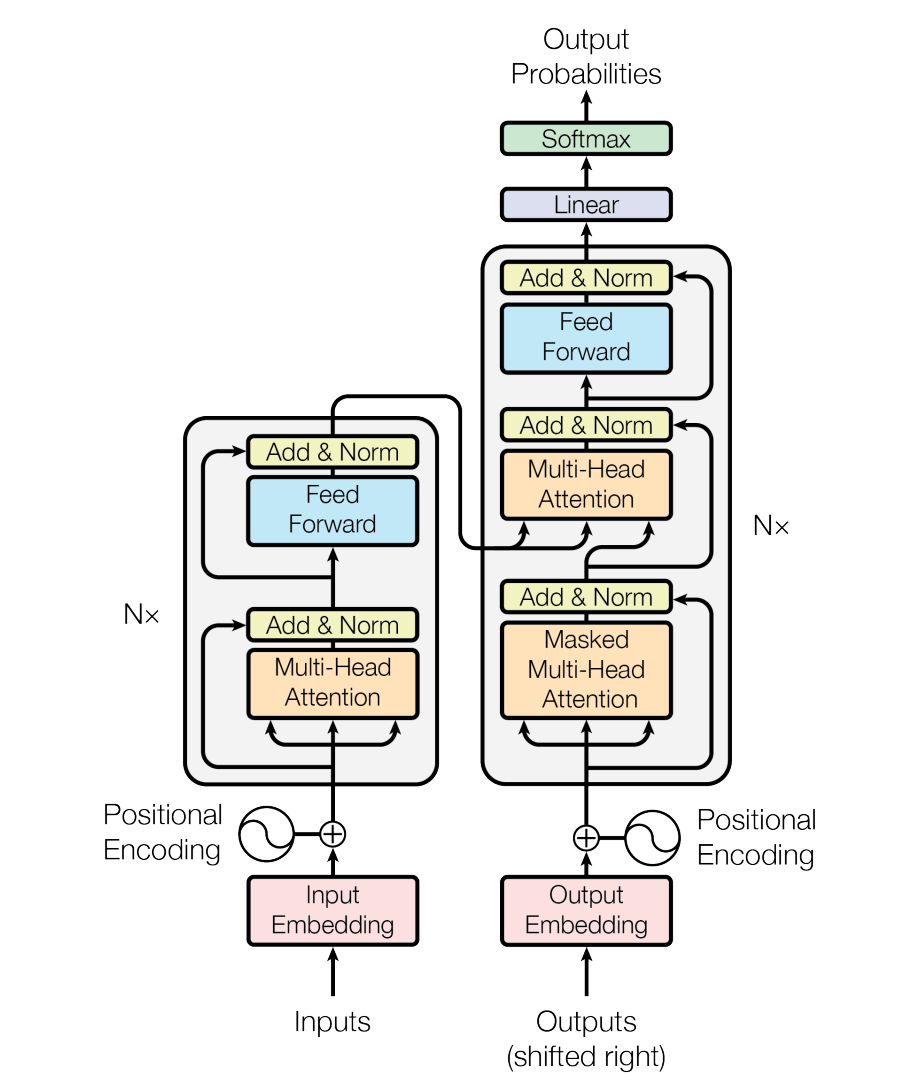
\includegraphics[width=0.6\textwidth]{Figures/Transformer.png}
    \caption{The Transformer-model architecture \cite{vaswani_attention_2023}}
    \label{fig:transformer_model}
\end{figure}

The positional embedding ensures that the model can interpret the position of the tokens within the sequence. The Multi-Head Attention block consist of linear mappings of query, key and value pairs which are run in parallel. The number of linear mappings computed per block is denoted as $h$. Thus, the attention function is performed on a set of queries and an attention matrix is computed \cite{vaswani_attention_2023}.

\subsubsection{Convolutional Block Attention Module (CBAM)}
The Convolutional Block Attention Module (CBAM) connects the attention paradigm with the convolutional approach and consists of two sub-modules. Inputs are convoluted, and with the first module, a 1D channel attention map on the convolution-channels is generated. Afterwards, these channel attentions are used as an input to the spatial attention module to compute the spatial attention. This means that the model is then able to learn which channels and which regions of the input data are more important than others. These two blocks can then be integrated within a convolutional based network or a residual based network.

\begin{figure}[H]
    \centering
    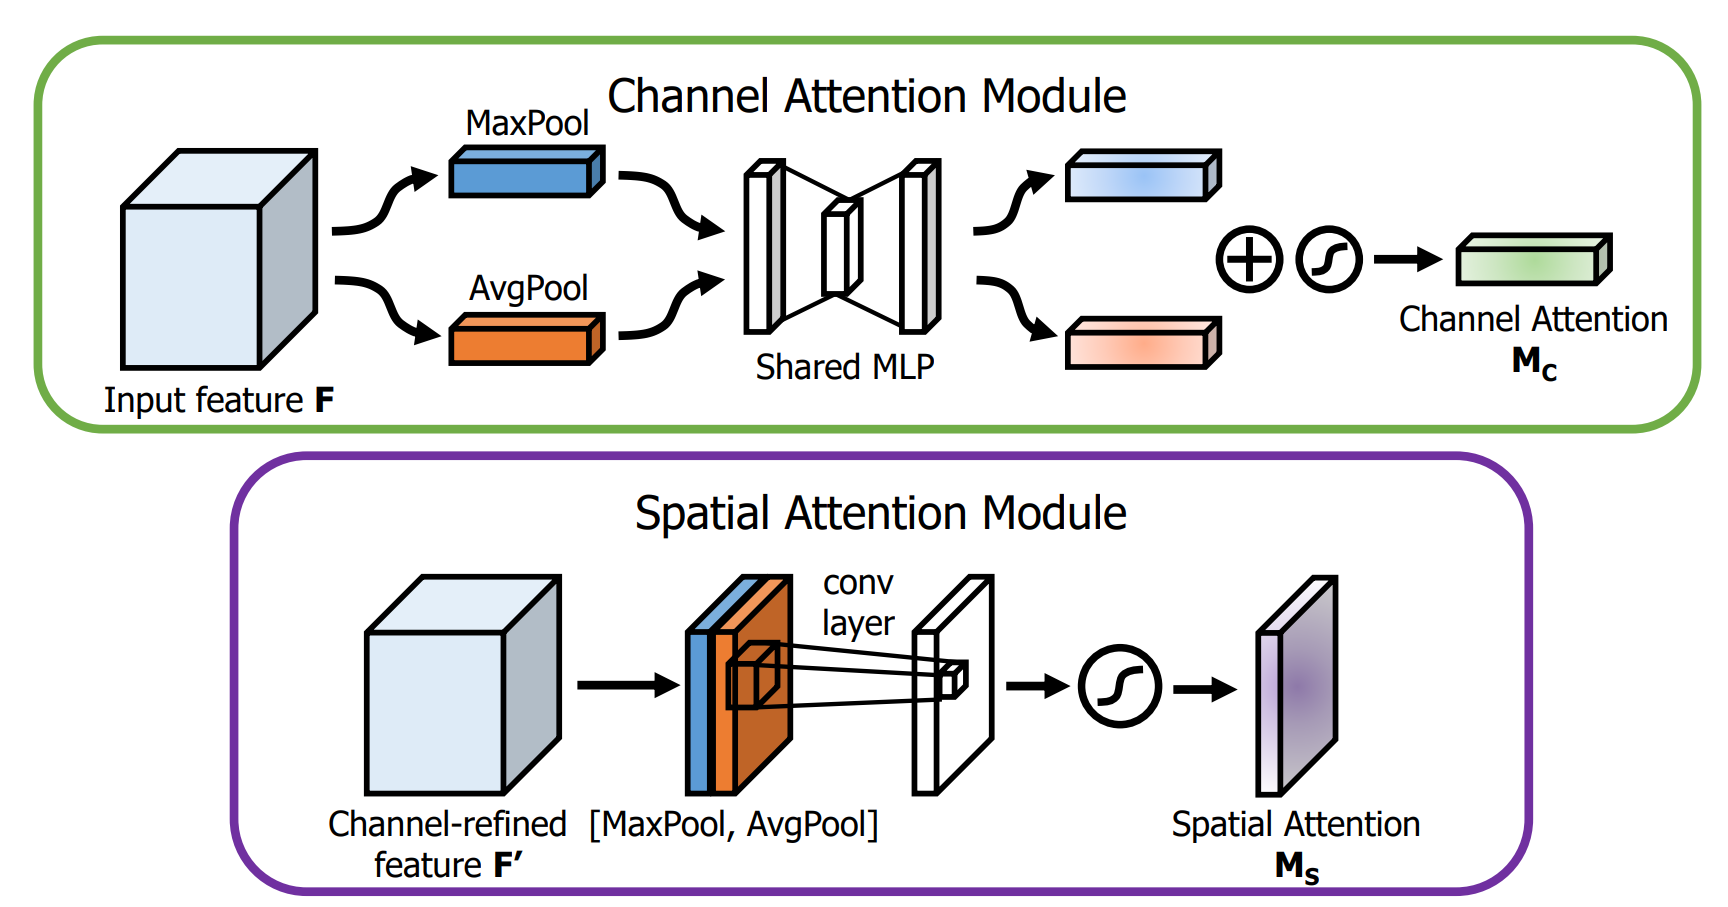
\includegraphics[width=0.8\textwidth]{Figures/cbam_modules.png}
    \caption{Channel \& Spatial attention module blocks \cite{woo_cbam_2018}}
    \label{fig:cbam_modules}
\end{figure}

\begin{figure}[H]
    \centering
    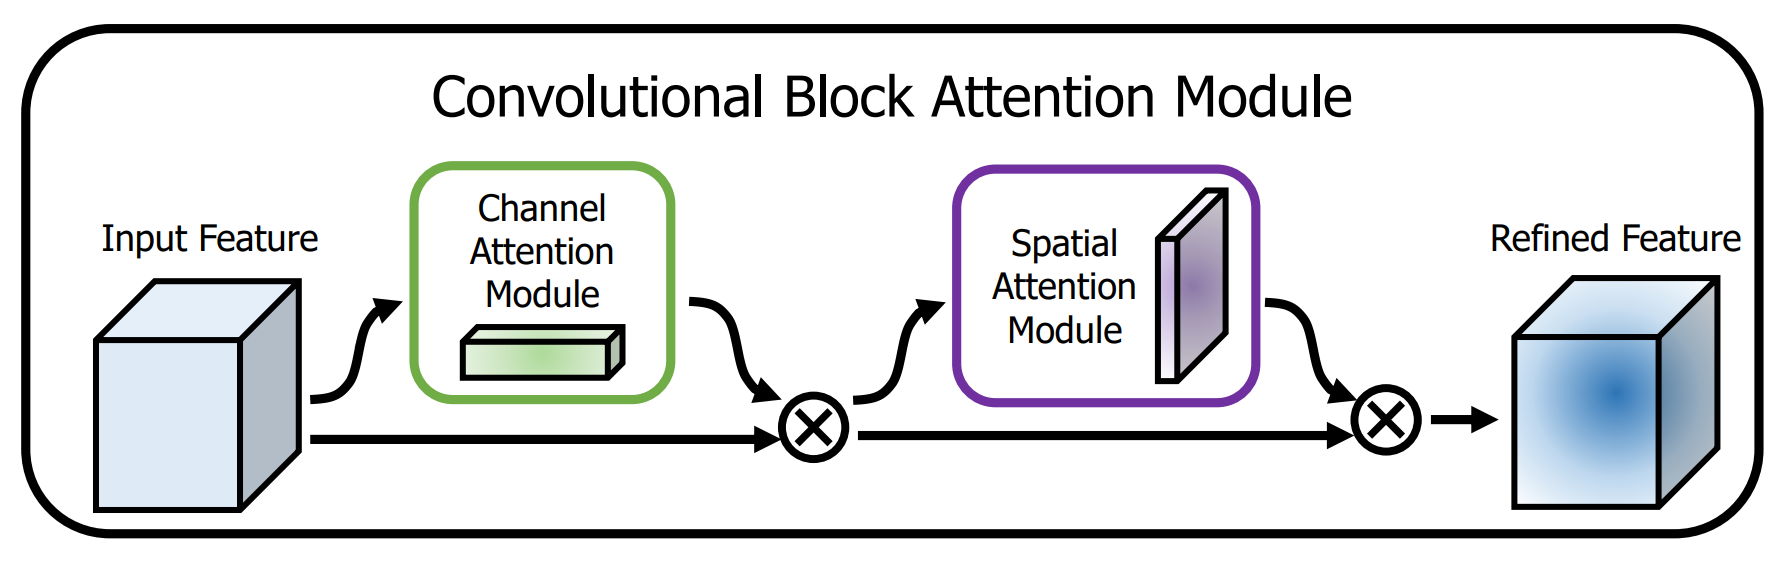
\includegraphics[width=0.7\textwidth]{Figures/cbam_modul.png}
    \caption{CBAM-architecture \cite{woo_cbam_2018}}
    \label{fig:cbam}
\end{figure}


\subsubsection{Vision Transformer (ViT)}
The Vision transformer model (ViT) has been recently published \cite{dosovitskiy_image_2021} and uses the mechanisms of Transformer-based models for computer vision tasks. Input data is divided into multiple patches of size n. A positional embedding is added and the embedded patches are then used as tokenized input to the transformer encoder. In the encoder, the patches are fed through $L$ subsequent Multi-Head Attention blocks. Lastly, the last encoder block outputs are fed into a MLP-Head which itself is connected to the output-layer representing the classes to be predicted.

\begin{figure}
    \centering
    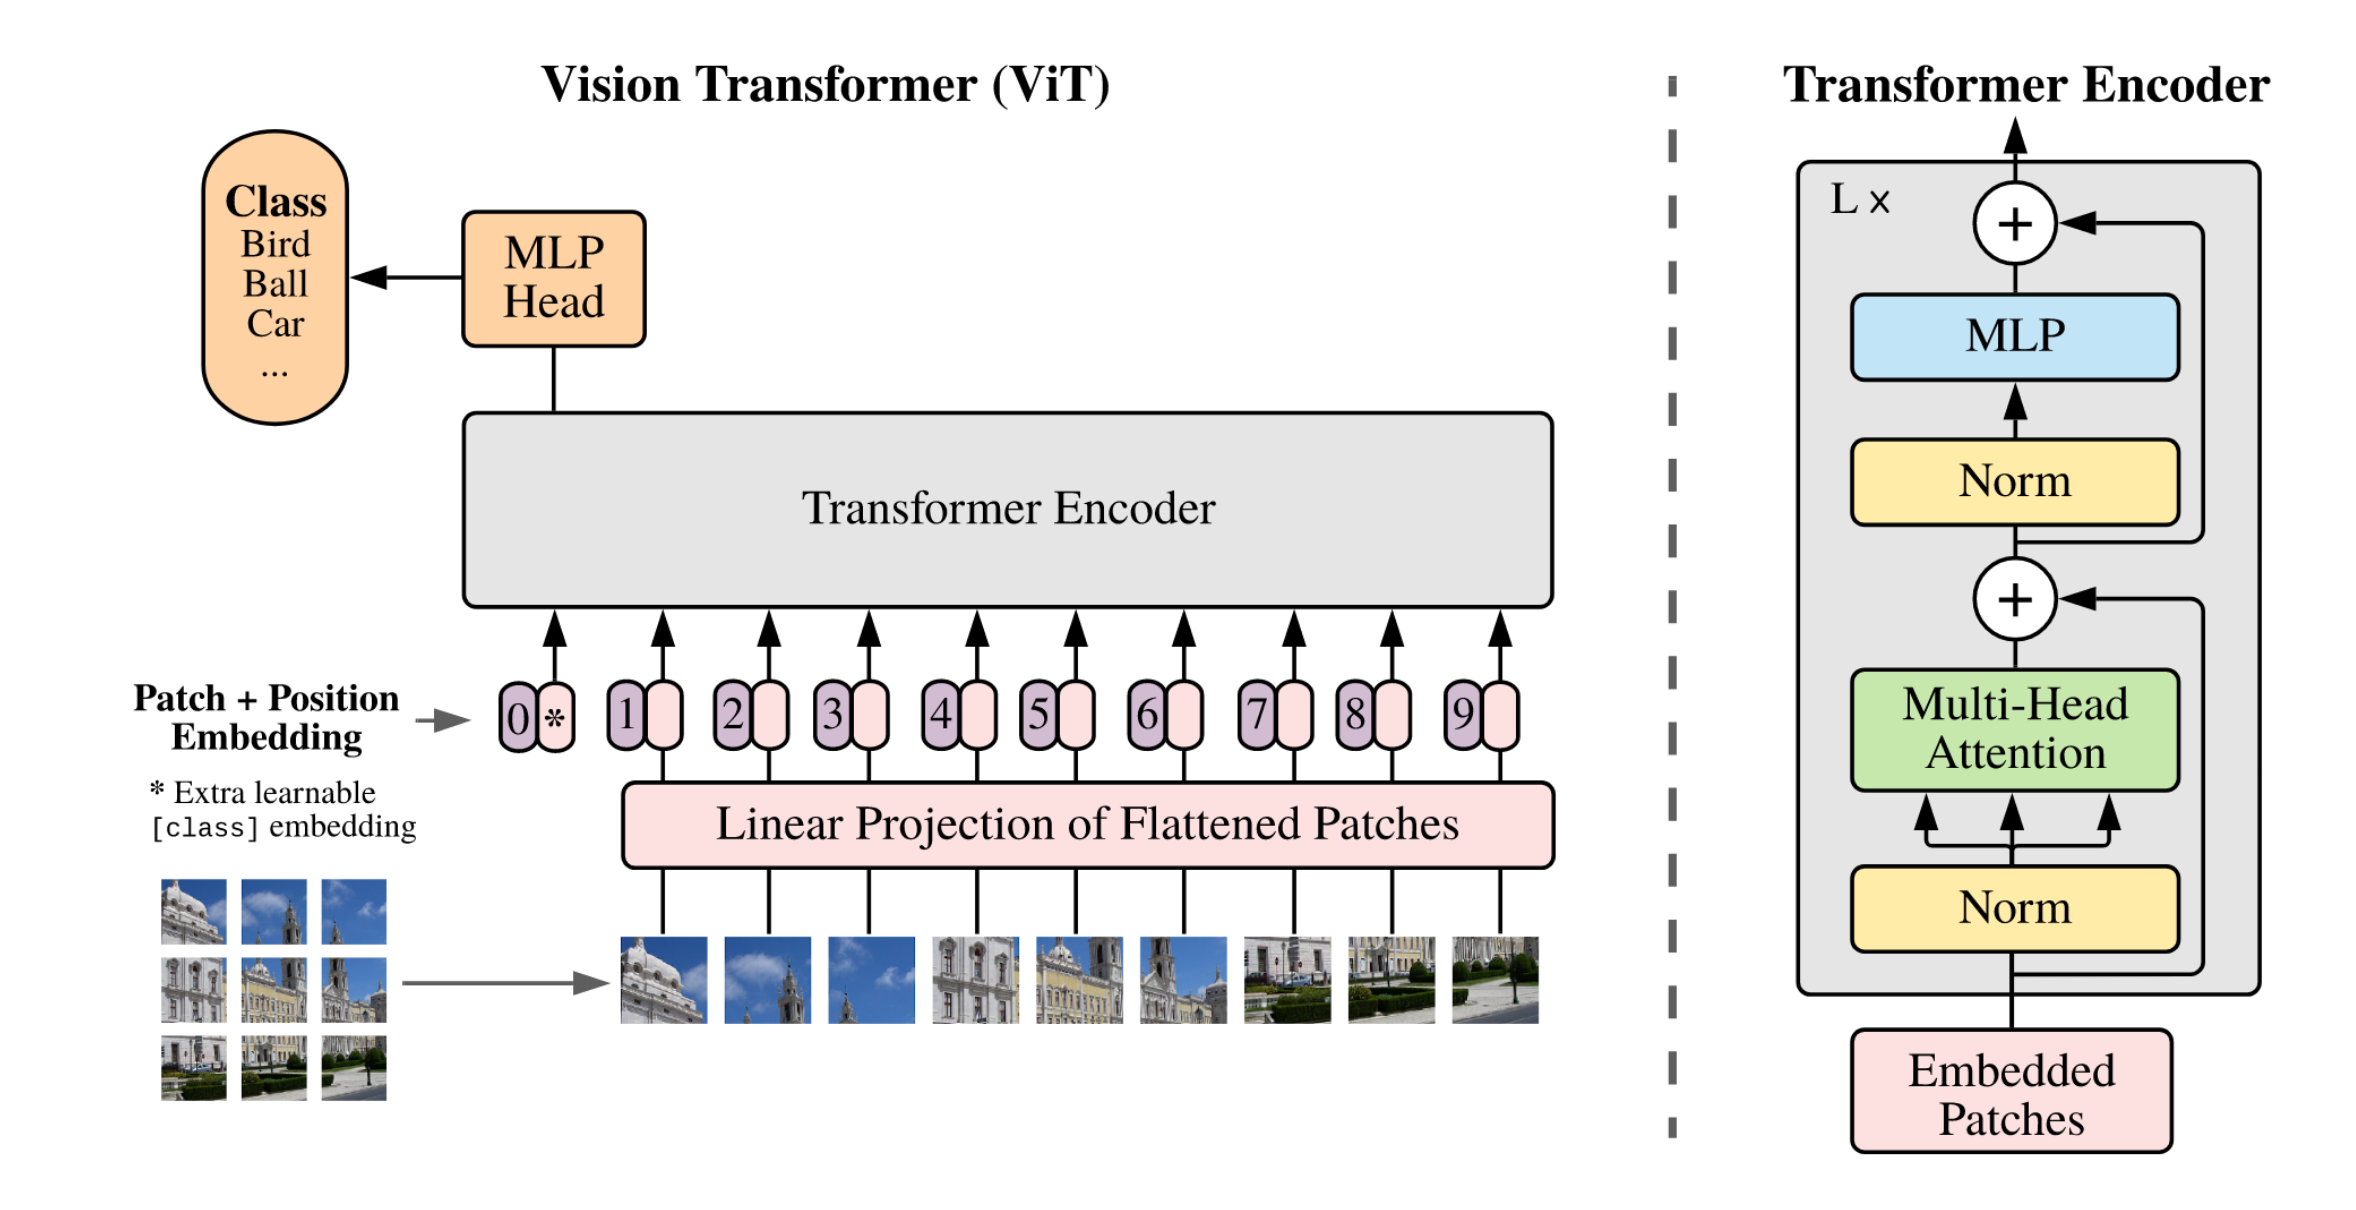
\includegraphics[width=\textwidth]{Figures/ViT.png}
    \caption{Vision Transformer \cite{dosovitskiy_image_2021}}
    \label{fig:vit_model}
\end{figure}

%----------------------------------------------------------------------------------------
 
% Indicate the main file. Must go at the beginning of the file.
% !TEX root = ../main.tex

%----------------------------------------------------------------------------------------
% CHAPTER TEMPLATE
%----------------------------------------------------------------------------------------


\chapter{Methods} % Main chapter title

\label{Chapter3} % Change X to a consecutive number; for referencing this chapter elsewhere, use \ref{ChapterX}

%----------------------------------------------------------------------------------------
% SECTION 1
%----------------------------------------------------------------------------------------

\section{Training Data}



%-----------------------------------
% SUBSECTION 1
%-----------------------------------
\subsection{Data simulation}

The spectra were simulated with the Software Sessa v2.2.0 developed by Smekal et al. It uses binding energies from the NIST database and inelastic mean free paths (IMFPs) from various publications and simulations to calculate the spectra. Since version 2.2.0, it also accounts for energy dependence of the IMFP \cite{noauthor_nist_2010}.

As the probing depth of XPS is around 10 nanometers and the information diminishes rapidly after the first few nanometers, the thicknesses used for simulation of the top layer are n $\in$ [1, 2, 3, 4, 5] nm. A second simulation approach was to simulate slow transitions of elements such as seen in migration or alloying processes. As shown in 

\includegraphics[]{}

The spectra simulated are using two components from all elements (n=81), thus 6561 permutations. With the 5 thicknesses, we obtain 32805 spectra for each experimental setup. To achieve a similar carbon and oxide content as experimental data (because of environmental influences), there is a carbon and oxide layer with thickness of triangular distribution (12-24, mode 15) Angstrom on top. 


Sessa v2.2.0, Python-Wrapper, Databases of Sessa, etc., X-Y-axis, carbon / oxygen layer, etc.

%-----------------------------------
% SUBSECTION 2
%-----------------------------------

\subsection{Data preprocessing}

Each spectra was max-normalized using equation \ref{eqn:normalize} 

\begin{equation}
    x' = \frac{x}{max(x)}
\label{eqn:normalize}
\end{equation}

%----------------------------------------------------------------------------------------
% SECTION 2
%----------------------------------------------------------------------------------------

\section{Test Data}

There are multiple sources for test-data of XPS-spectra. A main database was found on XPSlibrary, provided by TXL. Further, the XPSSurfA on CMSS Hub from the Australian University La Trobe contains more than 1700 spectra of which >100 survey spectra were used for the evaluation of the model.


\subsection{Data preprocessing}

As is typical for data acquired from laboratories, XPS data comes in various formats and measurement parameters. Apart from XPS-specific parameters, the resolution and the range mostly influence the evaluation of spectra with deep-learning framework. Thus, an automated workflow for the spectra pre-processing is introduced to provide an entry point to the model.
Although most wide-survey spectra are measured with a comparable energy-range, it should be identical to the training data. Thus, any signal outside the specified binding energy range (0-1000 eV) is cut off and the discrete measurement points inside the range are interpolated or subsampled by using a uniformly distributed sampling method to match 1024 points.  
% Indicate the main file. Must go at the beginning of the file.
% !TEX root = ../main.tex

%----------------------------------------------------------------------------------------
% CHAPTER TEMPLATE
%----------------------------------------------------------------------------------------

\chapter{Results and discussion} % Main chapter title
\label{Chapter4}
The approach of modelling spectra and training a neural network model on their structure-label relation is an inherently biased approach, as we add the prior assumption of the model to create accurate spectra. Although this is clearly not the preferred baseline, scarce availability of labelled data often forces one to accept trade-offs. Nevertheless, this does not immediately imply failure at our tasks, but more importantly strongly depends on the prior assumption of spectra modelling. The following structure resembles our tasks formulated in the \nameref{Chapter1}. For each task, a table with the respective models, datasets and accuracies is shown.

%----------------------------------------------------------------------------------------
% SECTION 1
%----------------------------------------------------------------------------------------
\section{Qualitative elemental identification of bilayer systems}
\subsection{Elemental identification}
% model performance
The model performance for the qualitative elemental identification is shown in Table \ref{tab:acc_qual}. The categorical accuracies were computed for the individual clean and the mixcont dataset. Because experimental data can contain contamination, we generally expect the mixcont dataset to make our model more robust in that respect.
During the model development, it was obvious that we are prone to overfitting the simulated data resulting in poor performance on test data. Especially, because we do not represent the experimental spectra with enough accuracy, we must make sure to focus on the robustness of the model. Thus, the obvious approach was to choose the most simple model which was able to train effectively without overfitting and before aiming at the highest accuracy rates. The models remained unchanged for the qualitative identification for all datasets. Thus, a total of 8 models were developed for task 1 - one of each model type for each layer and the models were trained on the three datasets. For each best performing model for each layer and dataset, the confusion matrices are shown.

\begin{table}[H]
    \centering
    \centerline{
    \begin{tabular}{c|c|c|c|c|c|c}
        Dataset & Layer & Model   & No. Parameters & Training set acc. & Validation set acc. & Test set acc.*    \\
        \hline 
        mixcont & top   & CNN     &  82.1 M        &    91.34      &    86.58       & 24.65          \\
        (n=272k)&       & CNN-DCT &  85.5 M        &    97.25      &    86.42       & 38.5           \\
                &       & CBAM    &  20.1 M        &   92.80       &    82.80       & 28.64          \\
                &       & ViT     &  25.8 K        &    79.92     &    82.69       &  52.56  \\
        \hdashline
                & bot   & CNN     &   82.1 M       &    89.05       &      79.64    &     45.12      \\
                &       & CNN-DCT &                &               &                &                 \\
                &       & CBAM    &                &               &                &                \\
                &       & ViT     &                &               &                &               \\
        \hline                                   
        clean   & top   & CNN     &                &               &                &            \\
        (n=65k)&       & CNN-DCT &                &               &                &            \\
                &       & CBAM    &                &               &                &            \\
                &       & ViT     &                &               &                &            \\
        \hdashline
                & bot   & CNN     &                &               &                &             \\
                &       & CNN-DCT &                &               &                &             \\
                &       & CBAM    &                &               &                &            \\
                &       & ViT     &                &               &                &            \\
    \end{tabular}}
    \caption{Categorical accuracies, and number of parameters of the models in respect to dataset and sample layer
    *Test Dataset n=\nelementalspectra}
    \label{tab:acc_qual}
\end{table}



\subsubsection{Top layer prediction}
The best model to predict the top layer element was the Vision Transformer-Model, with an accuracy on the test dataset of 52.56 \%. Figure \ref{fig:top_best_loss} shows the categorical crossentropy loss and categorical accuracy for the training (blue) and the validation (orange) datasets respectively. In the confusion matrix, we can see that in the test dataset, Iron (Fe) has been wrongly predicted as Lithium (Li) a total of 4 times, which are the most failures of any wrongly predicted elements. An approach would be to plot the attention of the model on Lithium and Iron spectrum data to investigate the reason behind. However, as shown in Figures \ref{att:Fe} and \ref{att:Li}, they are not similar at all, which suggests that the model lacks complexity as both cases overlap in the feature space. As the model only has 25.8k trainable parameters, this is very much possible. 

\begin{figure}[H]
    \centering
    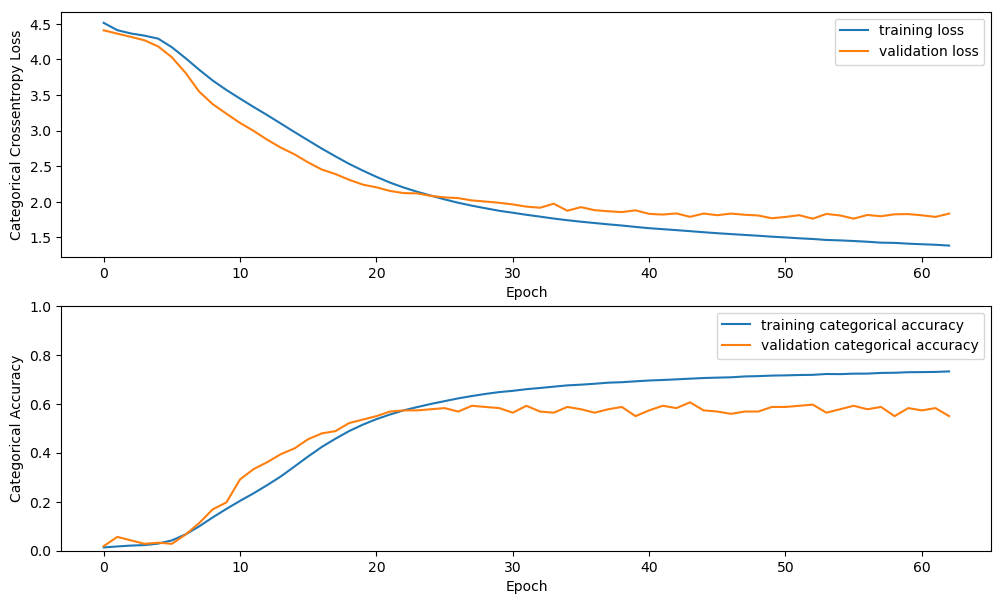
\includegraphics[width=\textwidth]{Figures/top_best_loss_acc_vit_4_32_3_4_64.png}
    \caption{Categorical crossentropy loss and crossentropy accuracy for the ViT model training on top-layer training data-labels}
    \label{fig:top_best_loss}
\end{figure}

\begin{figure}[H]
    \centering
    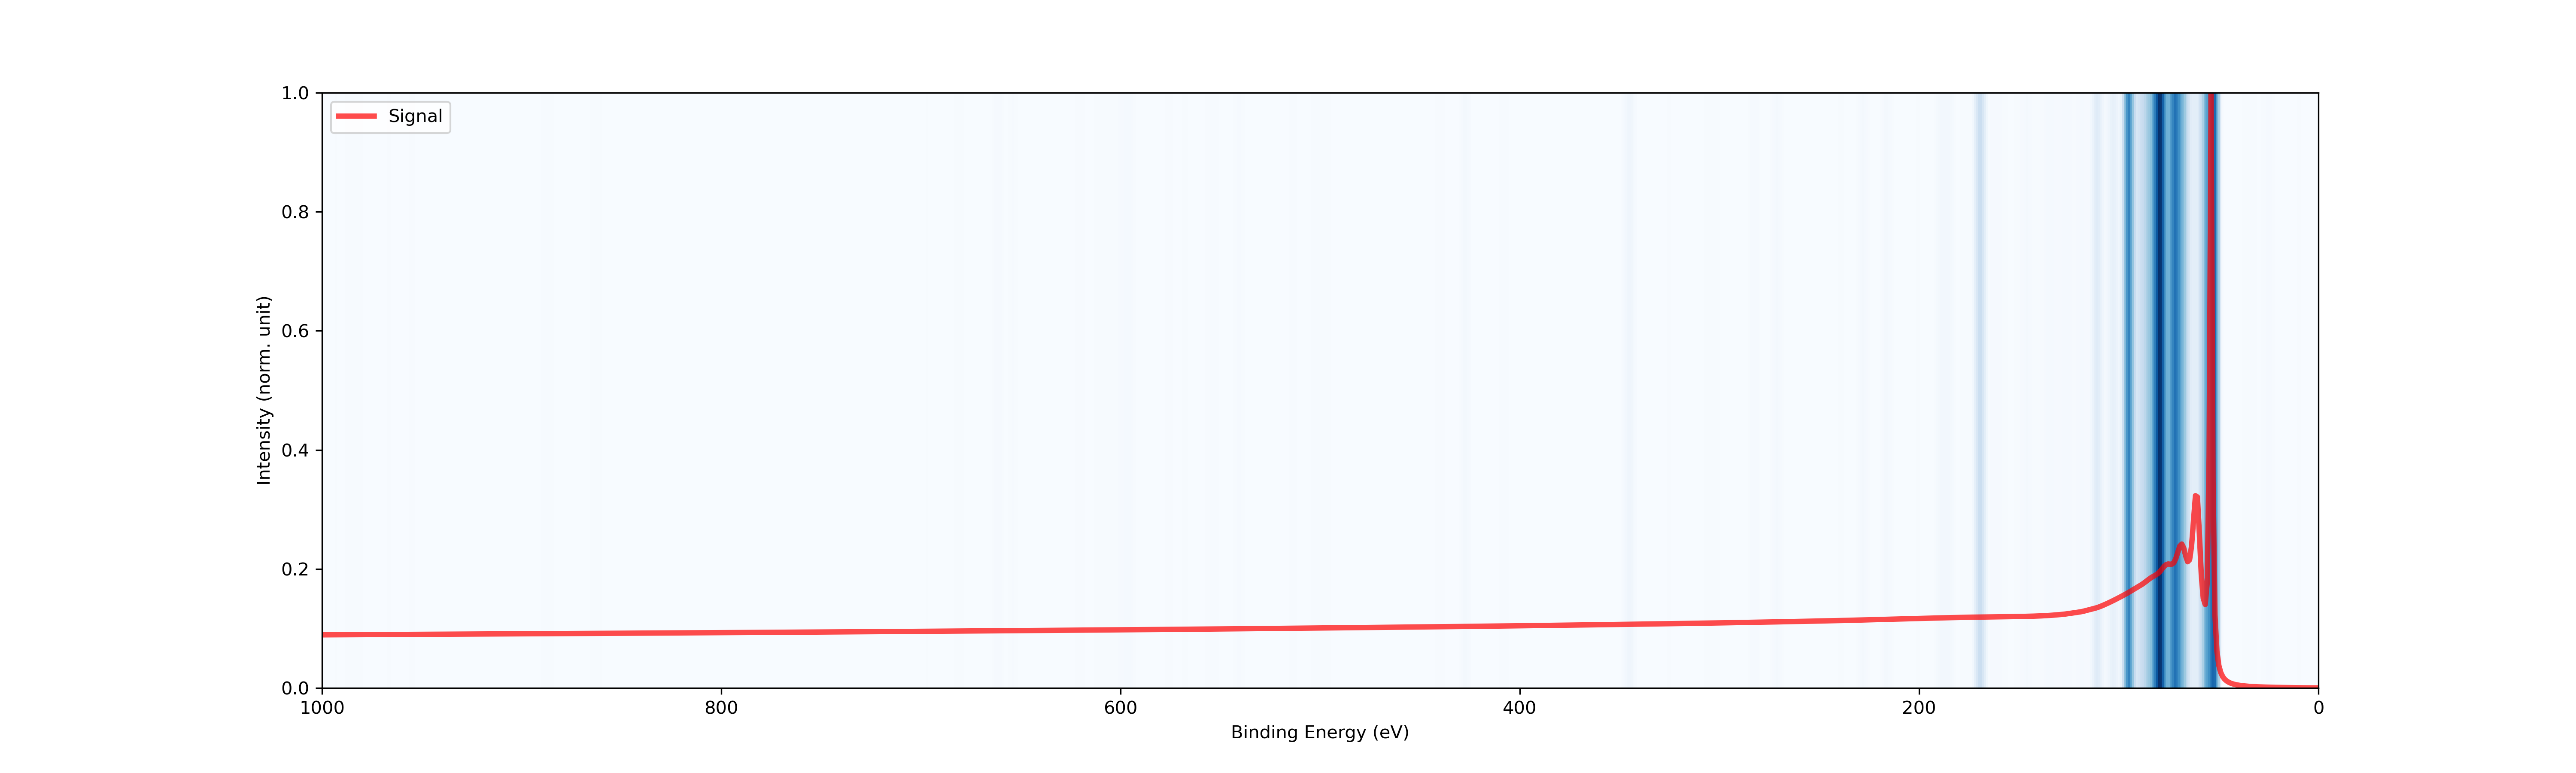
\includegraphics[width=\textwidth]{Figures/attention_map_Li.png}
    \caption{Attention map (blue) for the Lithium spectrum (red) prediction}
    \label{att:dy}
\end{figure}
\begin{figure}[H]
    \centering
    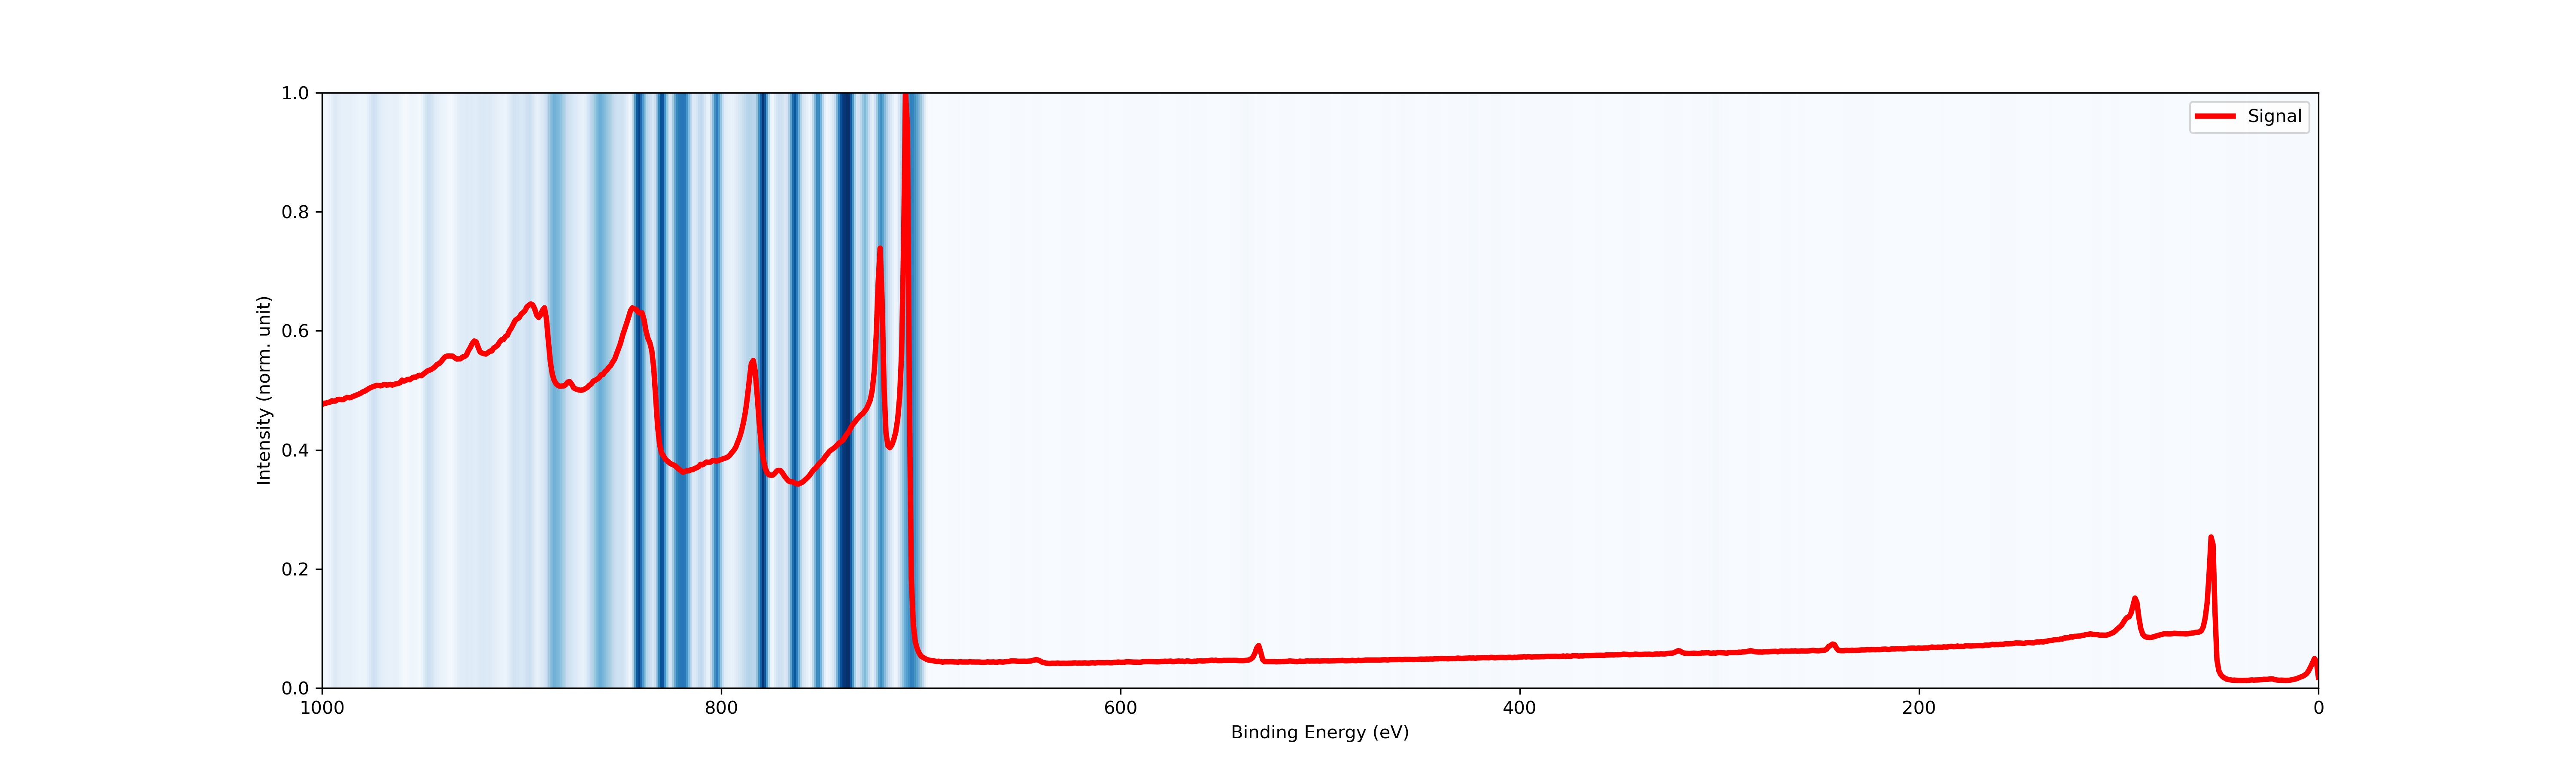
\includegraphics[width=\textwidth]{Figures/attention_map_Fe.png}
    \caption{Attention map (blue) for the Iron spectrum (red) prediction}
    \label{att:c}
\end{figure}




\begin{center}
\begin{figure}[H]
        \centerline{\includegraphics[width=1.4\textwidth]{Figures/best_task_1_model_CM.png}}
    \centering
    \caption{Confusion Matrix of Test-Data for best Top-Layer prediction}
    \label{cm_cnn_1l}
\end{figure}
\end{center}



\subsubsection{Bot layer prediction}


From the experimental data, the same test dataset was used as for the top-layer prediction. Because survey scans of buried layers are rare, we considered pure elemental spectra to be composed of a buried layer of the pure element respectively.
From Table \ref{tab:acc_qual}, we can see that the performance of the bottom layer prediction is not always lower than the top layer prediction. However, we would expect a lower accuracy for the bottom layer, due to the principle of XPS measurement, as electrons from the deeper layer must travel through the top layer and thus will be less intense and more influenced by scattering from interactions. Anyway, as we consider experimental data from pure elements as a two-layer system in our test-set, it could also be that the simulated spectra from buried pure elements actually resembles ground truth more accurately.




\subsection{Depth profile determination of native oxides and elements}

% As there's almost no test data this is experimental
Depth profiling or determination of overlayer thickness is often conducted in scientific experiments. However, data is usually not publicly available - and if - it does often not include survey spectra. This is because these measures are usually done with ion-sputtering profiling or angle-resolved measurements and as these experiments are time-consuming, only the regions of interests (where the peaks are expected depending on the sample) are scanned.
As depth profiling data is not readily available from public databases, the datasets obtained internally as explained in chapter \ref{exp_depth}, were used to evaluate the model on experimental data.
% model performance

\begin{table}[H]
    \centering
    \begin{tabular}{c|c|c|c|c}
        Dataset & Model   & No. Parameters & Training Dataset    & Validation Dataset    \\
        \hline
 mixcont+oxides& CNN     &                &                       &                         \\
               & CNN-DCT &                &                       &                         \\
               & CBAM    &                &                       &                         \\
               & ViT     &                &                       &                         \\

    \end{tabular}
    \caption{ and number of Parameters of the models in respect to dataset and layer}
    \label{tab:acc_depth}
\end{table}

% experimental data (AG_AG etc.)




%----------------------------------------------------------------------------------------
% SECTION 2
%----------------------------------------------------------------------------------------
\section{Elemental quantification of single layer systems}

% model performance
The model performance for the quantitative assessment of chemical composition is shown in Table \ref{tab:acc_quant}. The mean squared errors were computed for the multi dataset for each model.
% experimental data (AG_AG etc.)
From all experimental data, $\nmultispectra$ elemental spectra were used for the quantitative prediction. 

\begin{table}[H]
    \centering
    \begin{tabular}{c|c|c|c|c|c}
       Dataset & Model   & No. Parameters & Training dataset & Validation dataset*  & Test dataset*    \\
        \hline
        multi  & CNN     &   9.1 M        &     35.5       &   25.95                 &  1.92      \\
               & CNN-DCT &  35.3 M        &    13.61          &    14.16            &    3.83   \\
               & CBAM    & 28.2 M         &    23.32         &    14.94             &  2.68   \\ % CBAM_512_3_ES_MAE_4
               & ViT     &   35.3 M     &    33.81       &      34.86    &   2.68        \\
    \end{tabular}
    \caption{Number of parameters and threshold accuracy of the models}
    \label{tab:acc_quant}
\end{table}

As the threshold accuracy represents the percentage of elements with >10\% proportional content correctly quantified within a $\pm$10\% relative margin, it can be well compared to an experienced researchers result. With a maximum threshold accuracy of 3.83\% however, we are far off a good result for our best model. The full prediction mapped as heatmap is shown in Figure \ref{fig:multi_best_model}

\begin{figure}
    \centering
    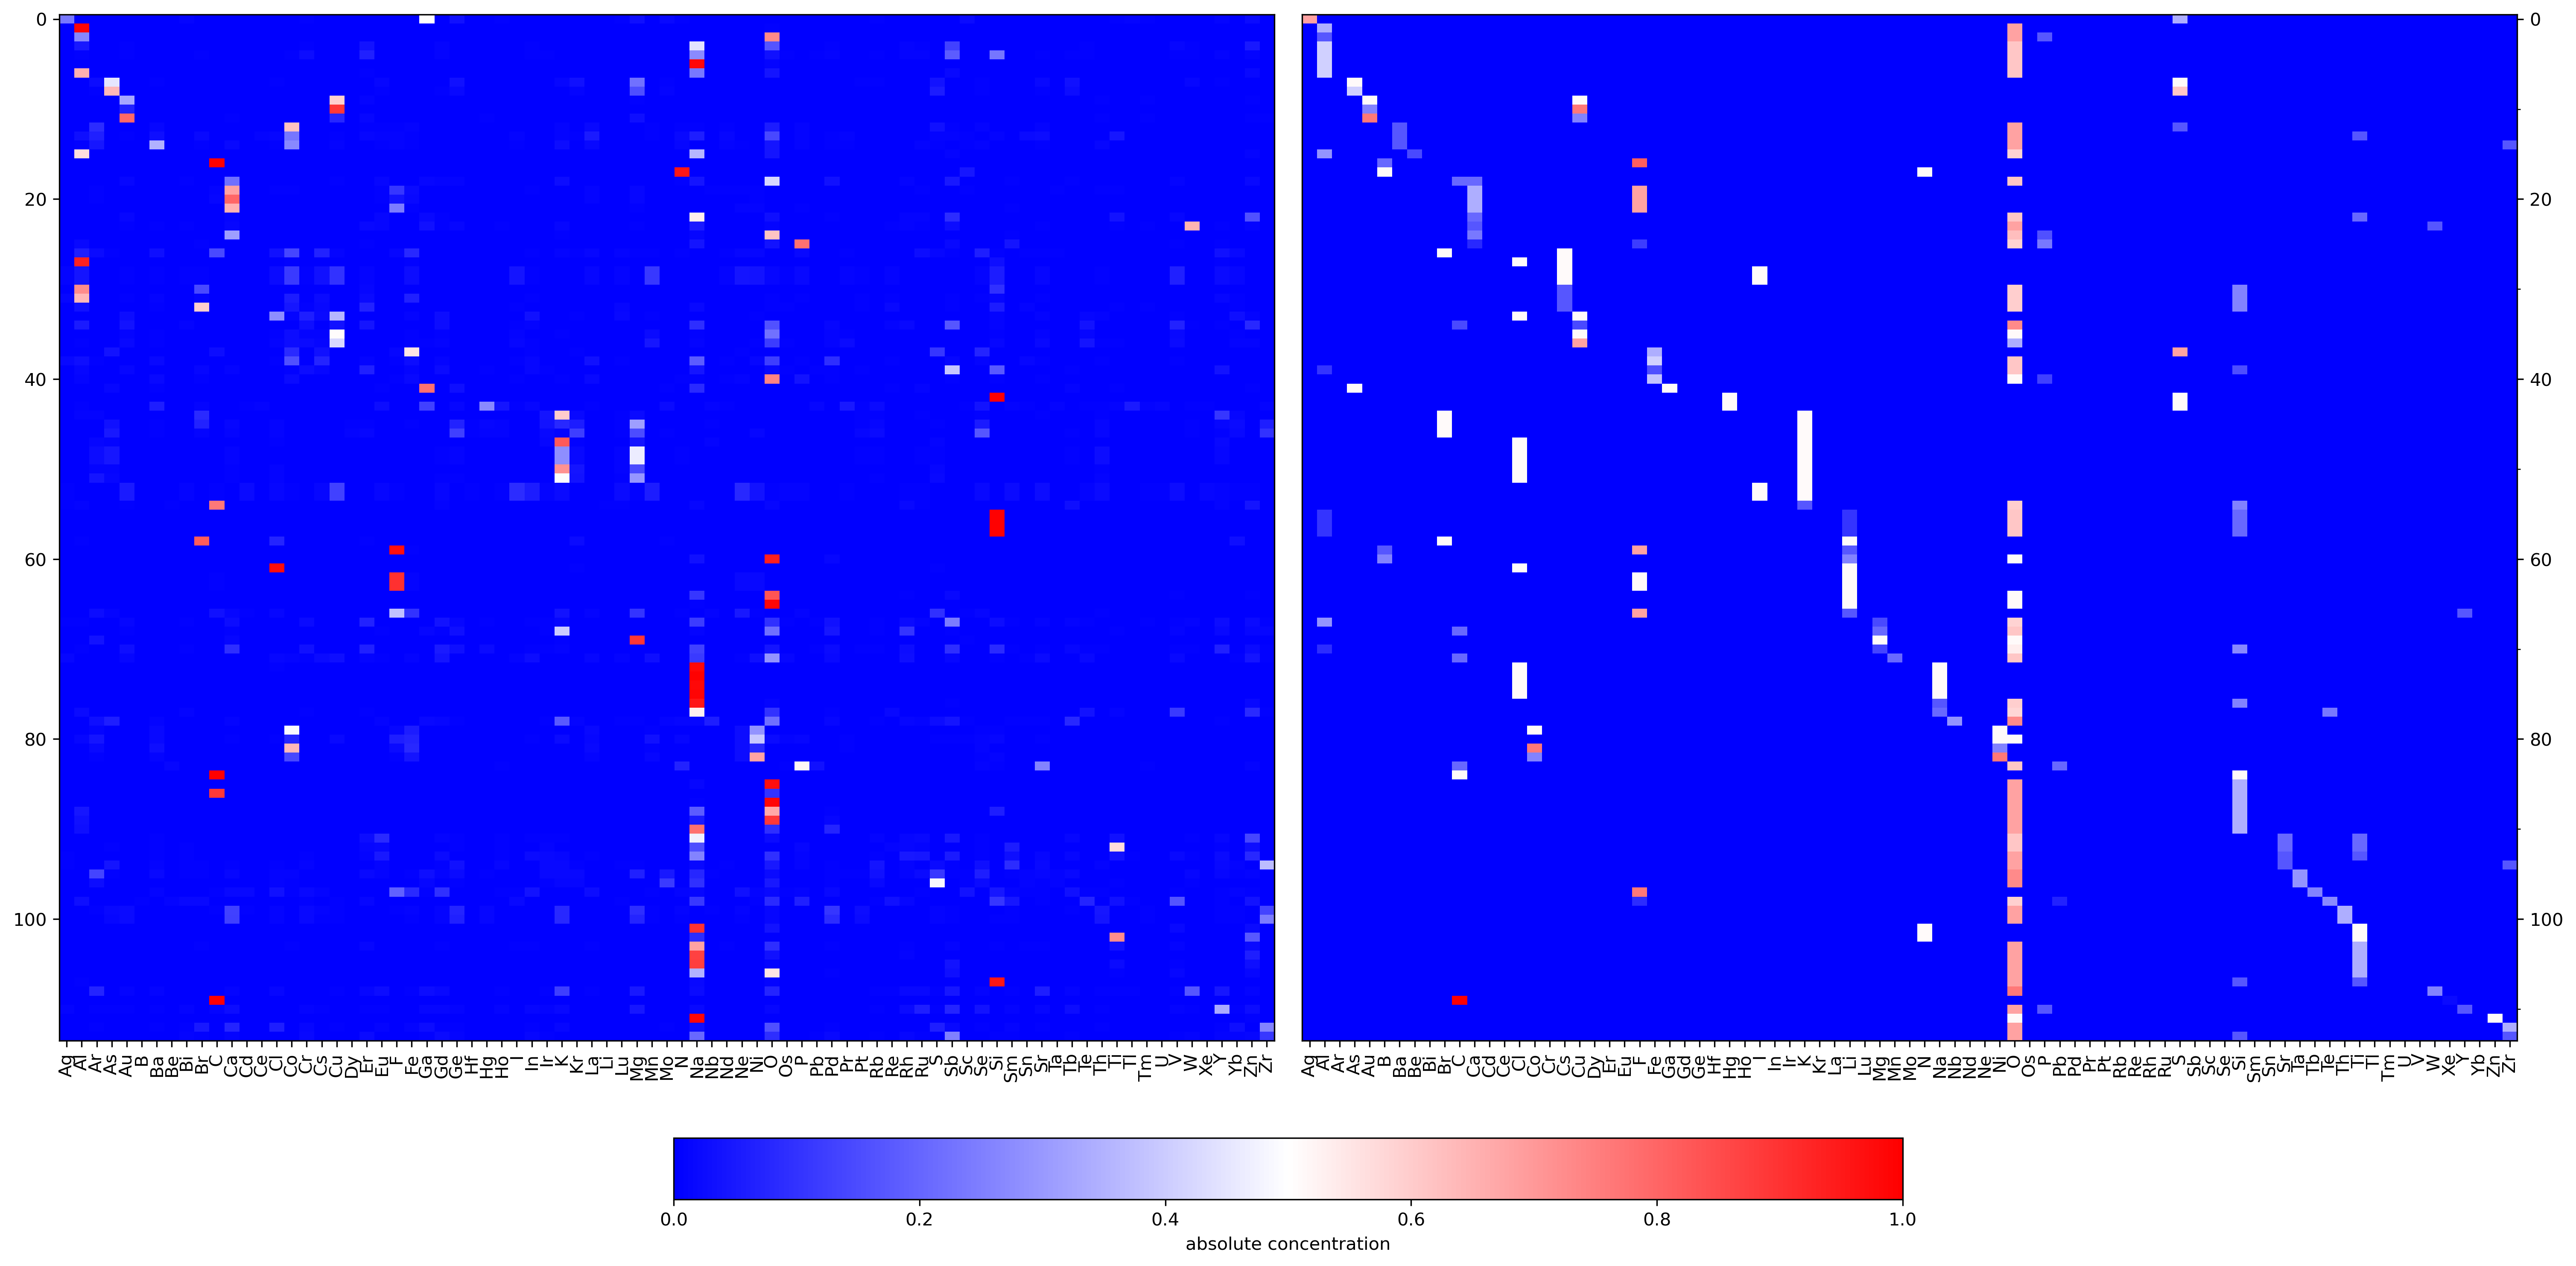
\includegraphics[width=\textwidth]{Figures/cnn_dct_mae_32F_multi_best_model_pred.png}
    \caption{The predictions of the best performing model on experimental multi-component data}
    \label{fig:multi_best_model}
\end{figure}

In contrast to previous studies on deep-learning assisted quantitative XPS analysis \cite{drera_deep_2019}, no relative sensitivity factors were applied in this approach. Furthermore, a significantly smaller training dataset of 30k versus the 100k which were used in their work. Lastly, the test data spectra they used were collected in experimental conditions and the training dataset was simulated according to the known conditions.

% plot visual attention feature


% Indicate the main file. Must go at the beginning of the file.
% !TEX root = ../main.tex

%----------------------------------------------------------------------------------------
% CHAPTER TEMPLATE
%----------------------------------------------------------------------------------------


\chapter{Conclusion} % Main chapter title

\label{Chapter5} % Change X to a consecutive number; for referencing this chapter elsewhere, use \ref{ChapterX}

%----------------------------------------------------------------------------------------
% SECTION 1
%----------------------------------------------------------------------------------------

\section{Main Section 1}


%-----------------------------------
% SUBSECTION 1
%-----------------------------------
\subsection{Subsection 1}

 


%----------------------------------------------------------------------------------------
% THESIS CONTENT - APPENDICES
%----------------------------------------------------------------------------------------
\appendix % Cue to tell LaTeX that the following "chapters" are Appendices

% Include the appendices of the thesis as separate files from the Appendices folder
% Uncomment the lines as you write the Appendices
% !TEX root = ../main.tex

%----------------------------------------------------------------------------------------
% APPENDIX A
%----------------------------------------------------------------------------------------

\chapter{Code} % Main appendix title

\label{AppendixA} % For referencing this appendix elsewhere, use \ref{AppendixA}

\section{Modules}

\subsection{Base module}
\label{code:base}
\lstinputlisting[language=Python]{Code/modules/base.py}

\subsection{Functions module}
\label{code:functions}
\lstinputlisting[language=Python]{Code/modules/functions_tf.py}

\subsection{Preprocessing module}
\label{preprocessing}
\lstinputlisting[language=Python]{Code/modules/preprocess.py}

\subsection{Prediction module}
\label{code:base}
\lstinputlisting[language=Python]{Code/modules/predict.py}

\subsection{Sessa Simulation module}
\label{Sessa_Module}
\lstinputlisting[language=Python]{Code/modules/sessa_py.py}



\section{Notebooks}

\subsection{NIST Chemical Shift Database Webscraper}
\label{NIST_WebScraper}
\lstinputlisting[language=Python]{Code/modules/req_async.py}

\subsection{XPSLibrary Webscraper}
\label{xpslibrary_webscraper}
\subsubsection*{Grab folders from XPSSurfA}\label{grab-folders-from-xpssurfa}

\begin{lstlisting}[language=Python]
from bs4 import BeautifulSoup
import os
import requests
import urllib.request
import os
\end{lstlisting}

\begin{lstlisting}[language=Python]
number = 1
URL = f'https://cmsshub.latrobe.edu.au/xpsdatabase/xpsrecords/download_data_files/{number}'
req = requests.get(URL)
soup = BeautifulSoup(open('../../data/test_data/XPSSurfA/view-source_https___cmsshub.latrobe.edu.au_xpsdatabase_xpsrecords.html'),
                            'html.parser')
numbers = [int(p.get('href').split('/')[-1]) 
           for p in soup.findAll(class_="html-attribute-value html-external-link") 
           if 'view' in p.get('href')]
\end{lstlisting}

\begin{lstlisting}[language=Python]
for number in numbers:
    print(number)
    if os.path.isfile(f'../../data/test_data/XPSSurfA/{number}.zip'):
        print('already downloaded')
        continue
    URL = f'https://cmsshub.latrobe.edu.au/xpsdatabase/xpsrecords/download_data_files/{number}'
    file_name  = f'../../data/test_data/XPSSurfA/{number}.zip'
    # Download the file from `url` and save it locally under `file_name`:
    with urllib.request.urlopen(URL) as response, open(file_name, 'wb') as out_file:
        data = response.read() # a `bytes` object
        out_file.write(data)
\end{lstlisting}

\subsubsection*{Unzip all downloaded files from
XPSSurfA}\label{unzip-all-downloaded-files-from-xpslibrary.com}

\begin{lstlisting}[language=Python]
import os
import zipfile

root_folder = '../../data/test_data/XPSSurfA'

# add //? before path if the path is too long otherwise it will throw an error

def extract_zip_files(root_folder):
    for foldername, subfolders, filenames in os.walk(root_folder):
        for filename in filenames:
            if filename.endswith('.zip'):
                zip_file_path = os.path.join(foldername, filename)
                print(os.path.join(foldername, os.path.splitext(filename)[0]))
                with zipfile.ZipFile(zip_file_path, 'r') as zip_ref:
                    zip_ref.extractall(os.path.join(foldername, os.path.splitext(filename)[0]))
\end{lstlisting}

\begin{lstlisting}[language=Python]
extract_zip_files(root_folder)
\end{lstlisting}

\subsubsection*{Check files from XPSSurfA}\label{check-files-from-xpssurfa}

\begin{lstlisting}[language=Python]
files = []
for foldername, subfolders, filenames in os.walk(root_folder):
    # check if there is a *.vms file in the folder
    # print(foldername)
    if any([filename.endswith('.vms') for filename in filenames]):
        # print('yes')
        files.append(([foldername + '\\' +filename for filename in filenames if filename.endswith('.vms')][0]))
\end{lstlisting}

\begin{lstlisting}[language=Python]
len(files) # we have 121 test files
\end{lstlisting}

\begin{lstlisting}
121
\end{lstlisting}

\begin{lstlisting}[language=Python]
files = [f for f in files if len(f.split('_')) > 2 and len(f.split('_')[-1]) < 15 and not 'Cali' in f]
\end{lstlisting}

\begin{lstlisting}[language=Python]
files
\end{lstlisting}

\begin{lstlisting}
['../../data/test_data/XPSSurfA\\10\\Fe_Fe.vms',
 '../../data/test_data/XPSSurfA\\13\\Ar_Ar.vms',
 '../../data/test_data/XPSSurfA\\149\\Cu_Cu_Ultra.vms',
 '../../data/test_data/XPSSurfA\\15\\Mg_Mg.vms',
 '../../data/test_data/XPSSurfA\\150\\Ag_Ag_Ultra.vms',
 '../../data/test_data/XPSSurfA\\151\\Au_Au_Ultra.vms',
 '../../data/test_data/XPSSurfA\\154\\Nb_Nb.vms',
 '../../data/test_data/XPSSurfA\\16\\Ni_Ni.vms',
 '../../data/test_data/XPSSurfA\\17\\Mo_Mo.vms',
 '../../data/test_data/XPSSurfA\\18\\Ta_Ta.vms',
 '../../data/test_data/XPSSurfA\\2\\Au_Au.vms',
 '../../data/test_data/XPSSurfA\\20\\Al_Al.vms',
 '../../data/test_data/XPSSurfA\\22\\Si_Si.vms',
 '../../data/test_data/XPSSurfA\\3\\Ag_Ag.vms',
 '../../data/test_data/XPSSurfA\\4\\Pt_Pt.vms',
 '../../data/test_data/XPSSurfA\\5\\Cu_Cu.vms',
 '../../data/test_data/XPSSurfA\\7\\W_W.vms',
 '../../data/test_data/XPSSurfA\\9\\In_In.vms']
\end{lstlisting}


\subsection{Sessa Simulation Notebook}
\label{xpslibrary_webscraper}
\hypertarget{define-directories}{%
\section*{Define directories}\label{define-directories}}

\begin{lstlisting}[language=Python]
from sessa_py import Experiment, Layer
import os
import numpy as np
import matplotlib.pyplot as plt
import itertools
import pandas as pd
import random
import subprocess
import sys
sys.path.append('../../../modules/')
import base
from tqdm.notebook import tqdm

root_dir = r'C:\Users\kochk\Documents\Git_Repos\Github\deep_xps'
sessa_dir = r"C:\Program Files (x86)\Sessa v2.2.0\bin\\"
\end{lstlisting}

\begin{lstlisting}[language=Python]
elements_sym = base.load_elem()
\end{lstlisting}

\hypertarget{build-experiments}{%
\section*{Build experiments}\label{build-experiments}}

\hypertarget{experiments-for-permutations-of-elements-and-thicknesses}{%
\subsection*{Experiments for permutations of elements and
thicknesses}\label{experiments-for-permutations-of-elements-and-thicknesses}}

\begin{lstlisting}[language=Python]
thicknesses = [10,20,30,40,50]
\end{lstlisting}

\begin{lstlisting}[language=Python]
perms = list(itertools.permutations(elements_sym, 2))
\end{lstlisting}

\hypertarget{separate}{%
\subsection*{Separate}\label{separate}}

\begin{lstlisting}[language=Python]
# check if all files done and store not simulated files in a list
os.chdir(r'C:\Users\kochk\Documents\Git_Repos\Github\deep_xps\tasks\0\simulation')
perms = list(itertools.permutations(elements_sym, 2))

data_dir = '../../../data/simulation_data/depth_sep/'
files = os.listdir(data_dir)
not_sim = []
sim = []

for perm in perms:
    for thickness in thicknesses:
        if os.path.isfile(data_dir+f'{perm[0]}_{perm[1]}_{thickness}_separate_spectra.spcreg1.spc'):
            sim.append([perm, thickness])
        else:
            not_sim.append(perm)
\end{lstlisting}

\begin{lstlisting}[language=Python]
len(not_sim)
\end{lstlisting}

\begin{lstlisting}[language=Python]
exp_dir = 'sep_NO'
data_dir = rf'C:\Users\kochk\Documents\Git_Repos\Github\deep_xps\data\simulation_data\{exp_dir}'

for entry in tqdm(perms):
    for thickness in thicknesses:
        # go to next if file already exists
        if os.path.isfile(data_dir+f'\{entry[0]}_{entry[1]}_{thickness}_separate_spectra.spcreg1.spc'):
            continue
        else:
            f = Experiment([Layer(entry[0], 50), Layer(entry[1], thickness)],
                        name=f'{entry[0]}_{entry[1]}_{thickness}',
                        exp_dir=exp_dir,
                        root_dir=root_dir,
                        sessa_dir=sessa_dir,
                        contamination=None)
            f.simulate()
\end{lstlisting}

\hypertarget{experiments-for-oxidates-with-and-without-carbon-traces}{%
\subsection*{Experiments for oxidates with and without carbon
traces}\label{experiments-for-oxidates-with-and-without-carbon-traces}}

\begin{lstlisting}[language=Python]
oxides = [
        '/Be/O/',
        '/Mg/O/',
        '/B2/O3/',
        '/Al2/O3/',
        '/Si/O2/',
        '/Sc2/O3/',
        '/Ti/O2/',
        '/Cr2/O3/',
        '/Mn/O2/',
        '/Fe2/O3/',
        '/Co/O/',
        '/Ni/O/',
        '/Cu/O/',
        '/Zn/O/',
        '/Ga2/O3/',
        '/Ge/O2/',
        '/As2/O3/',
        '/Y2/O3/',
        '/Zr/O2/',
        '/Nb2/O5/',
        '/Mo/O3/',
        '/Ru/O2/',
        '/Rh2/O3/',
        '/Pd/O/',
        '/Ag/O/',
        '/Cd/O/',
        '/In2/O3/',
        '/Sn/O2/',
        '/Sb2/O3/',
        '/Te/O2/',
        '/Hf/O2/',
        '/Ta2/O5/',
        '/W/O3/',
        '/Re/O3/',
        '/Ir/O2/',
        '/Pt/O/',
        '/Au2/O3/',
        '/Hg/O/',
        '/Tl2/O3/',
        '/Pb/O/',
        '/Bi2/O3/',
]
\end{lstlisting}

\begin{lstlisting}[language=Python]
for entry in tqdm(oxides):
    for thickness in thicknesses:
        f = Experiment(
                       layers=[Layer(entry.split('/')[1], 50), Layer(entry, thickness)],
                       root_dir= root_dir,
                       sessa_dir= sessa_dir,
                       exp_dir= 'oxides_NO',
                       contamination=None,
                       shifts_probability=0.8,
                       overwrite=False
                       )
        f.simulate()
\end{lstlisting}

\begin{lstlisting}[language=Python]
for entry in tqdm(oxides):
    for thickness in thicknesses:
        f = Experiment(
                       layers=[Layer(entry.split('/')[1], 50), Layer(entry, thickness)],
                       root_dir= root_dir,
                       sessa_dir= sessa_dir,
                       exp_dir= 'oxides_CO',
                       contamination=True,
                       shifts_probability=0.8,
                       overwrite=False
                       )
        f.simulate()
\end{lstlisting}

\hypertarget{build-multi-layer-system-for-depth-profiling}{%
\subsection*{Build multi-layer system for
depth-profiling}\label{build-multi-layer-system-for-depth-profiling}}

\begin{lstlisting}[language=Python]
layer_thickness = 5 # Angstrom
grad_steps = layer_thickness
N_layers = 100 / grad_steps # 100 % divided by the gradient steps

def create_gradients(grad_steps, rev=False, N_layers=N_layers):
    gradient = np.arange(100+grad_steps, step=grad_steps)
    
    if rev is True: 
        rev_grad_matrix = np.repeat([np.flip(gradient)], axis=0, repeats=N_layers)
        for number, line in enumerate(rev_grad_matrix):
            if number == 0:
                continue
            rev_grad_matrix[number][-number:] = 0
        return rev_grad_matrix
    else:
        grad_matrix = np.repeat([gradient], axis=0, repeats=N_layers)
        for number, line in enumerate(grad_matrix):
            if number == 0:
                continue
            grad_matrix[number][-number:] = 0
        return grad_matrix
\end{lstlisting}

\begin{lstlisting}[language=Python]
rev = create_gradients(5, rev=True)
grad = create_gradients(5)
grad = np.arange(100+grad_steps, step=grad_steps) # 0 to 100 in steps of grad_steps
rev = np.flip(grad) # reverse the gradient
\end{lstlisting}

\begin{lstlisting}[language=Python]
iterator = tqdm(perms)
for elems in iterator:
    a = Experiment(
                name=f'{elems[0]}_{elems[1]}',
                layers=[(Layer(f'(/{elems[0]}/){grad[p]}(/{elems[1]}/){rev[p]}', thickness=5))
                        for p in range(len(grad))],
                root_dir=root_dir,
                sessa_dir=sessa_dir,
                exp_dir='grad_NO',
                etching=8,
                contamination=None)
    a.simulate()
\end{lstlisting}

\begin{lstlisting}[language=Python]
# elems[0] is the bulk, elem[1] is the top layer with variable thickness
for elems in tqdm(perms):
        for thickness in thicknesses:
                f = Experiment(name=f'{elems[0]}_{elems[0]}_{elems[1]}',
                       layers= [Layer(elems[0], 50), Layer(elems[0], elems[1])], 
                       root_dir=root_dir, 
                       sessa_dir=sessa_dir,
                       exp_dir='depth_CO_sep_new',
                       etching=None)
                f.simulate()
\end{lstlisting}

\hypertarget{check-if-all-files-done}{%
\subsubsection*{Check if all files done}\label{check-if-all-files-done}}

\begin{lstlisting}[language=Python]
for elems in perms:
    for thickness in thicknesses:
        path = not(os.path.isfile('..\data\simfiles\depth_CO_sep\{elems[0]}_{elems[1]}_{thickness}.txt'))
    if path:
        print(f'..\data\simfiles\depth_CO_sep\{elems[0]}_{elems[1]}_{thickness}.txt')
        break
\end{lstlisting}

\begin{lstlisting}[language=Python]
[(i, os.path.isfile(f'C:/Users/kochk/Documents/Git_Repos/Github/deep_xps/data/simfiles/depth_CO_sep_new/{elems[0]}_{elems[1]}.txt')) 
 for i, elems in enumerate(perms) 
 if not os.path.isfile(f'C:/Users/kochk/Documents/Git_Repos/Github/deep_xps/data/simfiles/depth_CO_sep_new/{elems[0]}_{elems[1]}.txt')]
\end{lstlisting}

\begin{lstlisting}[language=Python]
for i, elems in enumerate(perms):
    for thickness in thicknesses:
        if not os.path.isfile(f'C:/Users/kochk/Documents/Git_Repos/Github/deep_xps/data/simfiles/depth_CO_sep_new/{elems[0]}_{elems[1]}_{thickness}.txt'):
            print(i, elems, thickness)
\end{lstlisting}

\begin{lstlisting}[language=Python]
# remove files
path='../data/simulation_data/depth_CO_sep/'
for file in os.listdir(path):
    if len(file.split('_')) == 6:
        os.remove(os.path.join(path,file))
        print(f'{file} removed.')
\end{lstlisting}

\begin{lstlisting}[language=Python]
os.chdir(r'C:\Users\kochk\Documents\Git_Repos\Github\deep_xps\tasks\0\simulation')
\end{lstlisting}

\begin{lstlisting}[language=Python]
# check if all files done and store not simulated files in a list

data_dir = '../../../data/simulation_data/grad_NO/'
files = os.listdir(data_dir)
not_sim = []
sim = []
etching_rates = [100, 90, 80, 70, 60]
for perm in perms:
    for etching in etching_rates:
        if os.path.isfile(data_dir+f'{perm[0]}_{perm[1]}_{etching}_etching_spectra.spcreg1.spc'):
            sim.append([perm, etching])
        else:
            not_sim.append(perm)
not_sim = [f for f in not_sim if not "Xe" in f]
\end{lstlisting}

\begin{lstlisting}[language=Python]
not_sim = pd.Series(not_sim).unique()
\end{lstlisting}

\hypertarget{one-element-layers}{%
\subsection*{One-element layers}\label{one-element-layers}}

\begin{lstlisting}[language=Python]
for element in tqdm(elements_sym):
    if os.path.isfile(f'{root_dir}\\data\\simulation_data\\one_layer\\{element}_{element}_spectra.spc'):
        continue
    cmd_str = ['\\PROJECT LOAD SESSION "C:\Program Files (x86)\Sessa v2.2.0\\bin/Sessa_ini.ses"',
                    '\\SPECTROMETER SET RANGE 486.6:1486.6 REGION 1',
                    f'\\SAMPLE SET MATERIAL {element}',
                    # f'\\SAMPLE ADD LAYER /C/O/ THICKNESS {int(random.triangular(12, 24, 15))} ABOVE 0',
                    '\\MODEL SET CONVERGENCE 1.000e-02',
                    '\\MODEL SET SE true',
                    '\\MODEL SIMULATE',
f'\\MODEL SAVE SPECTRA "{root_dir}\\data\\simulation_data\\one_layer\\{element}_{element}_spectra.spc"']
    with open(f'{root_dir}\\data\\simfiles\\one_layer\\{element}_{element}.txt', 'w') as f:
        f.writelines('\n'.join(cmd_str))
    filename_abs = f'{root_dir}\\data\\simfiles\\one_layer\\{element}_{element}.txt'
    os.chdir(sessa_dir)
    SWHIDE = 0
    info = subprocess.STARTUPINFO()
    info.dwFlags = subprocess.STARTF_USESHOWWINDOW
    info.wShowWindow = SWHIDE
    p = subprocess.Popen('sessa.exe -s "%s"' % filename_abs, startupinfo=info)
    p.wait()
\end{lstlisting}

\hypertarget{mixture-compounds}{%
\section*{Mixture compounds}\label{mixture-compounds}}

\begin{lstlisting}[language=Python]
from base import get_combinations

folder = 'multi_one_layer'
data_dir = rf'C:\Users\kochk\Documents\Git_Repos\Github\deep_xps\data\simulation_data\{folder}'
perms = get_combinations(elements_sym, number_of_layers=1, number_of_combinations=30_000, lower=2, upper=4) # get one layer
thickness = [random.choice([10,20,30,40,50]), 50] # two-layer systems always have second layer of 50 Angstrom
for entry in tqdm(list(perms)[0]):
    print(f'\t Going for entry {entry} with thickness {thickness}')
    exp = Experiment(layers=[Layer(entry[i] , thickness[i]) for i in range(len(entry))],
            exp_dir=folder,
            root_dir=root_dir,
            sessa_dir=sessa_dir,
            contamination=False,
            shifts_probability=0.6)
    exp.simulate()
\end{lstlisting}


\subsection{Training dataset creation \& preprocessing}
\label{train_data_generation}
\hypertarget{import-and-prepare}{%
\section{Import and prepare}\label{import-and-prepare}}

\begin{lstlisting}[language=Python]
import sys
import re
import glob
import pandas as pd
import numpy as np
import pickle
from sklearn.model_selection import train_test_split
from sklearn.preprocessing import MultiLabelBinarizer

sys.path.append('../../modules') # add own modules
import preprocess, predict, functions_tf, base
\end{lstlisting}

\begin{lstlisting}[language=Python]
mlb, elements = base.retreive_mlb_and_elements()
n_elements = len(elements)
test_size_ratio = 0.2
\end{lstlisting}

\hypertarget{training-data-for-top-bot-layer}{%
\section{Training Data for top bot
layer}\label{training-data-for-top-bot-layer}}

\hypertarget{mixcont}{%
\subsection{mixcont}\label{mixcont}}

\begin{lstlisting}[language=Python]
folders = [
            'grad_CO',              # depth-profiles with CO-adv.       with gradient layers
            'grad_CO_med',          # depth with 6 angstrom CO-adv.       with gradient layers
            'grad_NO',              # depth-profiles without CO-adv.    with gradient layers
            'sep_CO',               # depth-profiles with CO-adv.       with separated layers
            'sep_CO_med',           # depth with 6 angstrom CO-adv.       with separated layers
            'sep_NO',               # depth-profiles without CO-adv.    with separated layers
            'one_layer_CO',         # one-layer simulations with CO-adv.
            'one_layer_CO_med',     # one-layer simulations with 6 angstrom CO-adv.
            'one_layer',            # one-layer simulations
            ]

files = [file for file in glob.glob(f'../../data/simulation_data/{folders[0]}/*.spc')]
for folder in folders[1:]:
    files.extend([file for file in glob.glob(f'../../data/simulation_data/{folder}/*.spc')])
\end{lstlisting}

\begin{lstlisting}[language=Python]
print(len(files))
\end{lstlisting}

\begin{lstlisting}
194649
\end{lstlisting}

\begin{lstlisting}[language=Python]
(32400*6) + (3*81)
\end{lstlisting}

\begin{lstlisting}
194643
\end{lstlisting}

\begin{lstlisting}[language=Python]
df = pd.concat([pd.read_csv(file,
                            sep='\s+', header=None, skiprows=1,
                            usecols=[1],
                            names=['_'.join(file.split('\\')[1].split('_')[:-1])]).T 
                                    for file in files]).T
df.to_pickle('../../data/df_mixcont.pkl') # save the df without preprocessing
\end{lstlisting}

\hypertarget{preprocess}{%
\subsubsection{preprocess}\label{preprocess}}

\begin{lstlisting}[language=Python]
df = pd.read_pickle('../../data/df_mixcont.pkl') 
\end{lstlisting}

\begin{lstlisting}[language=Python]
df_norm = preprocess.MaxScale_df(df).reset_index(drop=True)  # each spectrum is scaled to 1
# reduce size to 1024 and add relative noise
df_noise = df_norm[::2].apply(lambda x: x+x*np.random.normal(0, np.random.randint(1,3)*0.01 , len(x)))
df_scaled = df_noise.T
df_scaled = df_scaled.dropna()
df_scaled = df_scaled.T.reset_index(drop=True)
\end{lstlisting}

\begin{lstlisting}[language=Python]
df_scaled.to_pickle('../../data/df_mixcont_scaled.pkl')  # save the normalized, scaled df
\end{lstlisting}

\hypertarget{top-layer-data}{%
\subsubsection{Top Layer data}\label{top-layer-data}}

\begin{lstlisting}[language=Python]
df_scaled = pd.read_pickle('../../data/df_mixcont_scaled.pkl')
\end{lstlisting}

\begin{lstlisting}[language=Python]
x_train, x_test, y_train, y_test = train_test_split(df_scaled.T.values,
                                # first part of the filename is the top label
                                df_scaled.columns.map(lambda x: x.split('_')[0]), 
                                test_size=0.3,
                                random_state=42)
\end{lstlisting}

\begin{lstlisting}[language=Python]
y_train = np.array([[mlb.transform([[y_train[i]]])[0]] 
                            for i in range(len(y_train))])
y_test = np.array([[mlb.transform([[y_test[i]]])[0]] 
                            for i in range(len(y_test))])
\end{lstlisting}

\begin{lstlisting}[language=Python]
data = {
        'name': 'two-layer and one-layer systems, top labels',
        'x_train': x_train,
        'x_test': x_test,
        'y_train': y_train,
        'y_test': y_test
}
\end{lstlisting}

\begin{lstlisting}[language=Python]
pickle.dump(data, open('../../data/training_data/1/dataset_mixcont_top_layer.pkl', 'wb'))
\end{lstlisting}

\hypertarget{bot-layer-data}{%
\subsubsection{Bot Layer data}\label{bot-layer-data}}

\begin{lstlisting}[language=Python]
df_scaled = pd.read_pickle('../../data/df_mixcont_scaled.pkl')
\end{lstlisting}

\begin{lstlisting}[language=Python]
x_train, x_test, y_train, y_test = train_test_split(df_scaled.T.values,
                                                    df_scaled.columns.map(lambda x: x.split('_')[1]), # second part of the filename is the bot label
                                                    test_size=0.3,
                                                    random_state=42)
\end{lstlisting}

\begin{lstlisting}[language=Python]
y_train = np.array([    
                        [
                            mlb.transform([[y_train[i]]])[0]
                        ] 
                            for i in range(len(y_train))
                        ])
y_test = np.array([ 
                       [
                            mlb.transform([[y_test[i]]])[0],
                       ] 
                            for i in range(len(y_test))
                        ])
\end{lstlisting}

\begin{lstlisting}[language=Python]
data = {
        'name': 'two-layer and one-layer systems, bot labels',
        'x_train': x_train,
        'x_test': x_test,
        'y_train': y_train,
        'y_test': y_test
}
\end{lstlisting}

\begin{lstlisting}[language=Python]
pickle.dump(data, open('../../data/training_data/1/dataset_mixcont_bot_layer.pkl', 'wb'))
\end{lstlisting}

\begin{lstlisting}[language=Python]
folders = [
            'grad_CO',              # depth-profiles with CO-adv.       with gradient layers
            'grad_CO_med',           # depth with 6 angstrom CO-adv.       with gradient layers
            'sep_CO',               # depth-profiles with CO-adv.       with separated layers
            'sep_CO_med',           # depth with 6 angstrom CO-adv.       with separated layers
            'one_layer_CO',         # one-layer simulations with CO-adv.
            'one_layer_CO_med',         # one-layer simulations with CO-adv.
            ]

files = [file for file in glob.glob(f'../../data/simulation_data/{folders[0]}/*.spc')]
for folder in folders[1:]:
    files.extend([file for file in glob.glob(f'../../data/simulation_data/{folder}/*.spc')])
\end{lstlisting}

\hypertarget{clean}{%
\subsection{clean}\label{clean}}

\begin{lstlisting}[language=Python]
folders = [
            'grad_NO',              # depth-profiles without CO-adv.    with gradient layers
            'sep_NO',               # depth-profiles without CO-adv.    with separated layers
            'one_layer',            # one-layer simulations
            ]

files = [file for file in glob.glob(f'../../data/simulation_data/{folders[0]}/*.spc')]
for folder in folders[1:]:
    files.extend([file for file in glob.glob(f'../../data/simulation_data/{folder}/*.spc')])
\end{lstlisting}

\begin{lstlisting}[language=Python]
df = pd.concat([pd.read_csv(file,
                            sep='\s+', header=None, skiprows=1,
                            usecols=[1],
                            names=['_'.join(file.split('\\')[1].split('_')[:-1])]).T 
                                    for file in files]).T
df.to_pickle('../../data/df_clean.pkl') # save the df without preprocessing
\end{lstlisting}

\hypertarget{preprocess}{%
\subsubsection{preprocess}\label{preprocess}}

\begin{lstlisting}[language=Python]
df = pd.read_pickle('../../data/df_clean.pkl') 
\end{lstlisting}

\begin{lstlisting}[language=Python]
df_norm = preprocess.MaxScale_df(df).reset_index(drop=True)  # each spectrum is scaled to 1
# reduce size to 1024 and add relative noise
df_noise = df_norm[::2].apply(lambda x: x+x*np.random.normal(0, np.random.randint(1,3)*0.01 , len(x)))
df_scaled = df_noise.T
df_scaled = df_scaled.dropna()
df_scaled = df_scaled.T.reset_index(drop=True)
\end{lstlisting}

\begin{lstlisting}[language=Python]
df_scaled.to_pickle('../../data/df_clean_scaled.pkl')  # save the normalized, scaled df
\end{lstlisting}

\hypertarget{top-layer-data}{%
\subsubsection{Top Layer data}\label{top-layer-data}}

\begin{lstlisting}[language=Python]
df_scaled = pd.read_pickle('../../data/df_clean_scaled.pkl')
\end{lstlisting}

\begin{lstlisting}[language=Python]
x_train, x_test, y_train, y_test = train_test_split(df_scaled.T.values,
                                                    df_scaled.columns.map(lambda x: x.split('_')[0]), # first part of the filename is the top label
                                                    test_size=test_size_ratio,
                                                    random_state=42)
\end{lstlisting}

\begin{lstlisting}[language=Python]
y_train = np.array([    
                        [
                            mlb.transform([[y_train[i]]])[0]
                        ] 
                            for i in range(len(y_train))
                        ])
y_test = np.array([ 
                       [
                            mlb.transform([[y_test[i]]])[0],
                       ] 
                            for i in range(len(y_test))
                        ])
\end{lstlisting}

\begin{lstlisting}[language=Python]
data = {
        'name': 'clean two-layer and one-layer systems, top labels',
        'x_train': x_train,
        'x_test': x_test,
        'y_train': y_train,
        'y_test': y_test
}
\end{lstlisting}

\begin{lstlisting}[language=Python]
pickle.dump(data, open('../../data/training_data/1/dataset_clean_top_layer.pkl', 'wb'))
\end{lstlisting}

\hypertarget{bot-layer-data}{%
\subsubsection{Bot Layer data}\label{bot-layer-data}}

\begin{lstlisting}[language=Python]
df_scaled = pd.read_pickle('../../data/df_clean_scaled.pkl')
\end{lstlisting}

\begin{lstlisting}[language=Python]
x_train, x_test, y_train, y_test = train_test_split(df_scaled.T.values,
                                                    df_scaled.columns.map(lambda x: x.split('_')[1]), # second part of the filename is the bot label
                                                    test_size=test_size_ratio,
                                                    random_state=42)
\end{lstlisting}

\begin{lstlisting}[language=Python]
y_train = np.array([    
                        [
                            mlb.transform([[y_train[i]]])[0]
                        ] 
                            for i in range(len(y_train))
                        ])
y_test = np.array([ 
                       [
                            mlb.transform([[y_test[i]]])[0],
                       ] 
                            for i in range(len(y_test))
                        ])
\end{lstlisting}

\begin{lstlisting}[language=Python]
data = {
        'name': 'clean two-layer and one-layer systems, bot labels',
        'x_train': x_train,
        'x_test': x_test,
        'y_train': y_train,
        'y_test': y_test
}
\end{lstlisting}

\begin{lstlisting}[language=Python]
pickle.dump(data, open('../../data/training_data/1/dataset_clean_bot_layer.pkl', 'wb'))
\end{lstlisting}

\hypertarget{training-data-with-multi}{%
\section{Training Data with Multi}\label{training-data-with-multi}}

\hypertarget{load-data-and-build-dataframe}{%
\subsection{Load data and build
dataframe}\label{load-data-and-build-dataframe}}

\begin{lstlisting}[language=Python]
folders = [
            'multi_one_layer'
            ]

files = [file for file in glob.glob(f'../../data/simulation_data/{folders[0]}/*.spc')]
\end{lstlisting}

\begin{lstlisting}[language=Python]
# windows
df = pd.concat([pd.read_csv(file,
                            sep='\s+', header=None, skiprows=1,
                            usecols=[1],
                            names=['_'.join(file.split('\\')[1].split('_')[:-1])]).T 
                                    for file in files]).T
df.to_pickle('../../data/df_multi.pkl') # save the df without preprocessing
\end{lstlisting}

\hypertarget{preprocess}{%
\subsection{Preprocess}\label{preprocess}}

\begin{lstlisting}[language=Python]
df = pd.read_pickle('../../data/df_multi.pkl')
\end{lstlisting}

\begin{lstlisting}[language=Python]
df_norm = preprocess.MaxScale_df(df).reset_index(drop=True)                                                    # each spectrum is scaled to 1
df_pp_noise = df_norm[::2].apply(lambda x:  x+x*np.random.normal(0, np.random.randint(1,3)*0.01 , len(x)))     # reduce size to 1024 and add noise
df_scaled = df_pp_noise.T
df_scaled= df_scaled.dropna()
df_scaled = df_scaled.T.reset_index(drop=True)
\end{lstlisting}

\begin{lstlisting}[language=Python]
df_scaled.to_pickle('../../data/df_multi_scaled.pkl')  # save the normalized, scaled df
\end{lstlisting}

\hypertarget{transform-data}{%
\subsection{Transform data}\label{transform-data}}

\begin{lstlisting}[language=Python]
x_train, x_test, y_train, y_test = train_test_split(df_scaled.T.values,
                                                    df.columns.map(lambda x: x.split('_')[:-1]
                                                                   ).map(base.pair_list_to_tuples
                                                                         ).map(base.one_hot_encode_concentrations),
                                                    test_size=0.2,
                                                    random_state=42)
\end{lstlisting}

\begin{lstlisting}[language=Python]
y_train = np.array([[y_train[i]] for i in range(len(y_train))])
y_test =   np.array([[y_test[i]] for i in range(len(y_test))])
\end{lstlisting}

\begin{lstlisting}[language=Python]
data = {
        'name': 'mixed systems, one layer',
        'x_train': x_train,
        'x_test': x_test,
        'y_train': y_train,
        'y_test': y_test
}
\end{lstlisting}

\begin{lstlisting}[language=Python]
pickle.dump(data, open('../../data/dataset_multi.pkl', 'wb'))
\end{lstlisting}

\hypertarget{training-data-with-depth}{%
\section{Training Data with Depth}\label{training-data-with-depth}}

\begin{lstlisting}[language=Python]
folders = [
            'grad_CO',              # depth-profiles with CO-adv.       with gradient layers
            'grad_NO',              # depth-profiles without CO-adv.    with gradient layers
            'grad_CO_med',           # depth with 6 angstrom CO-adv.       with gradient layers
            'sep_CO',               # depth-profiles with CO-adv.       with separated layers
            'sep_NO',               # depth-profiles without CO-adv.    with separated layers
            'sep_CO_med',           # depth with 6 angstrom CO-adv.       with separated layers
            'one_layer_CO',         # one-layer simulations with CO-adv.
            'one_layer',            # one-layer simulations
            'oxides_NO',            # oxides without CO-adv.
            'oxides_CO'             # oxides with CO-adv.
            ]

files = [file for file in glob.glob(f'../../data/simulation_data/{folders[0]}/*.spc')]
for folder in folders[1:]:
    files.extend([file for file in glob.glob(f'../../data/simulation_data/{folder}/*.spc')])
\end{lstlisting}

\begin{lstlisting}[language=Python]
df = pd.concat([pd.read_csv(file,
                            sep='\s+', header=None, skiprows=1,
                            usecols=[1],
                            names=['_'.join(file.split('\\')[1].split('_')[:-1])]).T 
                                    for file in files]).T
df.to_pickle('../../data/training_data/df/df_mixcont_depth.pkl') # save the df without preprocessing
\end{lstlisting}

\begin{lstlisting}[language=Python]
duplicateRows = df[df.duplicated()]
\end{lstlisting}

\hypertarget{preprocess}{%
\subsubsection{preprocess}\label{preprocess}}

\begin{lstlisting}[language=Python]
df = pd.read_pickle('../../data/training_data/df/df_mixcont_depth.pkl') 
\end{lstlisting}

\begin{lstlisting}[language=Python]
df_norm = preprocess.MaxScale_df(df).reset_index(drop=True)  # each spectrum is scaled to 1
# reduce size to 1024 and add relative noise
df_noise = df_norm[::2].apply(lambda x: x+x*np.random.normal(0, np.random.randint(1,3)*0.01 , len(x)))
df_scaled = df_noise.T
df_scaled = df_scaled.dropna()
df_scaled = df_scaled.T.reset_index(drop=True)
\end{lstlisting}

\begin{lstlisting}[language=Python]
df_scaled.to_pickle('../../data/training_data/df/df_mixcont_depth_scaled.pkl')  # save the normalized, scaled df
\end{lstlisting}

\begin{lstlisting}[language=Python]
df_scaled = pd.read_pickle('../../data/training_data/df/df_multi_scaled.pkl')
\end{lstlisting}

\begin{lstlisting}[language=Python]
layer_number = 5 # for the depth-profiling simplified in 5 categories: 0-10, 10-20, 20-30, 30-40, 40-50 Angstrom
gradient_bool: bool = False # is a measurement a gradient or not?
layers = [10, 20, 30, 40, 50]

def transform_depth_label(label):
    '''
    Map the concentration to the corresponding label between 0 and 1
    100, 90, 80, 70, 60 Etching
    100, 90, 80, 70, 60, Angstrom
    '''
    import math
    
    regex = re.compile('_[A-Za-z]+O')
    if regex.search(label) is not None:
        depth = label.split('_')[2]
        layer_thickness = (layers.index(int(depth))) / (len(layers)-1)
            
    if len(label.split('_')) < 4:
        top, bot, depth = label.split('_')
        gradient = 0
    else:
        top, bot, depth, gradient = label.split('_')
    # gives top, bottom, etching-depth, where top starts at 100% (with 0 etching) on the top
    if gradient == 'separate':
        # gradient = False
        gradient = 0
        layer_thickness = (layers.index(int(depth))) / (len(layers)-1)
    else:
        # gradient = True
        gradient = 1
        depth = int(depth)
        if depth <= 60:
            layer_thickness = 0.0
        elif depth > 100:
            layer_thickness = 1.0
        else:
            layer_thickness = (depth - 60) / 40.0

    return np.array([layer_thickness])
\end{lstlisting}

\begin{lstlisting}[language=Python]
x_train, x_test, y_train, y_test = train_test_split(df_scaled.T.values,
                                                    df_scaled.columns.map(lambda x: transform_depth_label(x)).to_numpy(), # first part of the filename is the top label
                                                    test_size=test_size_ratio,
                                                    random_state=42)
\end{lstlisting}

\begin{lstlisting}[language=Python]
y_train = np.array([[y_train[i][0]] for i in range(len(y_train))])
y_test =   np.array([[y_test[i][0]] for i in range(len(y_test))])
\end{lstlisting}

\begin{lstlisting}[language=Python]
data = {
        'name': 'depth profile labels',
        'x_train': x_train,
        'x_test': x_test,
        'y_train': y_train,
        'y_test': y_test,
}
\end{lstlisting}

\begin{lstlisting}[language=Python]
pickle.dump(data, open('../../data/dataset_depth.pkl', 'wb'))
\end{lstlisting}

\begin{lstlisting}[language=Python]
# gradient
x_train, x_test, y_train, y_test = train_test_split(df_scaled.T.values,
                                                    df_scaled.columns.map(lambda x: int('etching' in x)), # first part of the filename is the top label
                                                    test_size=test_size_ratio,
                                                    random_state=42)
\end{lstlisting}

\begin{lstlisting}[language=Python]
data = {
        'name': 'gradient labels',
        'x_train': x_train,
        'x_test': x_test,
        'y_train': y_train,
        'y_test': y_test,
}
pickle.dump(data, open('../../data/dataset_gradient.pkl', 'wb'))
\end{lstlisting}


\subsection{Test dataset creation \& preprocessing}
\label{train_data_generation}
\begin{lstlisting}[language=Python]
import matplotlib.pyplot as plt
import pandas as pd
import sys
sys.path.append('../../modules')
import preprocess
import pathlib as pl
\end{lstlisting}

\hypertarget{experimental-data}{%
\section*{Elemental data}\label{experimental-data}}

\begin{lstlisting}[language=Python]
import os
path = pl.Path('../../data/test_data/Selected_Spectra/elemental/')
elemental_exp = os.listdir(path)
\end{lstlisting}

\begin{lstlisting}[language=Python]
# concatenate all elemental spectra into one dataframe
import numpy as np
exp_df = pd.DataFrame()
for file in elemental_exp:
    filepath = os.path.join(path, file)
    try:
        x, y, x_new, y_new, label = preprocess.parse_file(filepath, filetype='vms', scale=True, N_points=1024)
    except: continue
    if x_new is not None:
        exp_df = pd.concat([exp_df, pd.DataFrame(np.flip(y_new), columns=['_'.join(label)])], axis=1)
\end{lstlisting}

\begin{lstlisting}[language=Python]
exp_df.shape
\end{lstlisting}

\begin{lstlisting}
(1024, 215)
\end{lstlisting}

\begin{lstlisting}[language=Python]
exp_df # 213 spectra with elemental composition
exp_df.to_pickle('../../data/experimental_data_elemental.pkl')
\end{lstlisting}

\hypertarget{multi-component-data}{%
\section*{Multi Component data}\label{multi-component-data}}

\begin{lstlisting}[language=Python]
import os
path = pl.Path('../../data/test_data/Selected_Spectra/multi/')
multi_exp = os.listdir(path)
\end{lstlisting}

\begin{lstlisting}[language=Python]
# concatenate all elemental spectra into one dataframe
import numpy as np
import base
exp_df = pd.DataFrame()
spectra = np.array
for i, file in enumerate(multi_exp):
    filepath = os.path.join(path, file)
    try:
        x, y, x_new, y_new, label = preprocess.parse_file(filepath, filetype='vms', scale=True, N_points=1024)
    except: continue
    if label == []: 
        print(file)
        continue
    if x_new is not None:
        if i == 0:
            spectra = np.flip(np.array([y_new]))
            labels = np.array(base.one_hot_encode_concentrations(label))
        else:
            spectra = np.append(spectra, np.flip(np.array([y_new])), axis=0)
            labels = np.append(labels, np.array(base.one_hot_encode_concentrations(label)), axis=0)
            
labels = labels.reshape(spectra.shape[0], 81)
\end{lstlisting}

\begin{lstlisting}[language=Python]
# spectra with multi composition
import pickle
pickle.dump([spectra, labels], open('../../data/experimental_data_multi.pkl', 'wb'))
\end{lstlisting}

\hypertarget{depth-profile}{%
\section*{Depth profile}\label{depth-profile}}

\begin{lstlisting}[language=Python]
from vamas import Vamas
import numpy as np
import os
dirs = r'C:\Users\kochk\Documents\Git_Repos\Github\deep_xps\data\test_data\Selected_Spectra\gradient_thickness'
files = os.listdir(dirs)
\end{lstlisting}

\begin{lstlisting}[language=Python]
exp_df = pd.DataFrame()
for file in files:
    x, y, x_new, y_new, label = preprocess.parse_file(os.path.join(dirs, file), 
                                                      filetype='vms',
                                                      scale=True,
                                                      N_points=1024)
    exp_df = pd.concat([exp_df, pd.DataFrame(np.flip(y_new), columns=[str('_'.join(label)+'_'+file.split('_')[2]+'_separate')])], axis=1)
exp_df.shape
\end{lstlisting}

\begin{lstlisting}
(1024, 7)
\end{lstlisting}


\begin{lstlisting}[language=Python]
exp_df # 213 spectra with elemental composition
exp_df.to_pickle('../../data/depth_profile.pkl')
\end{lstlisting}


\begin{lstlisting}[language=Python]
label
\end{lstlisting}


\section{Training Notebook}
\subsection{Task 1}
\input{Code/1/}
\subsection{Task 2}
\input{Code/2/}
\subsection{Task 3}
\input{Code/2/}


\section{Prediction Notebook}
\subsection{Task 1}
\input{Code/1/}
\subsection{Task 2}
\input{Code/2/}
\subsection{Task 3}
\input{Code/2/}

% !TEX root = ../main.tex

%----------------------------------------------------------------------------------------
% APPENDIX TEMPLATE
%----------------------------------------------------------------------------------------

\chapter{Confusion matrices} % Main appendix title

\label{AppendixB} % Change X to a consecutive letter; for referencing this appendix elsewhere, use \ref{AppendixX}


\begin{center}
\begin{figure}
        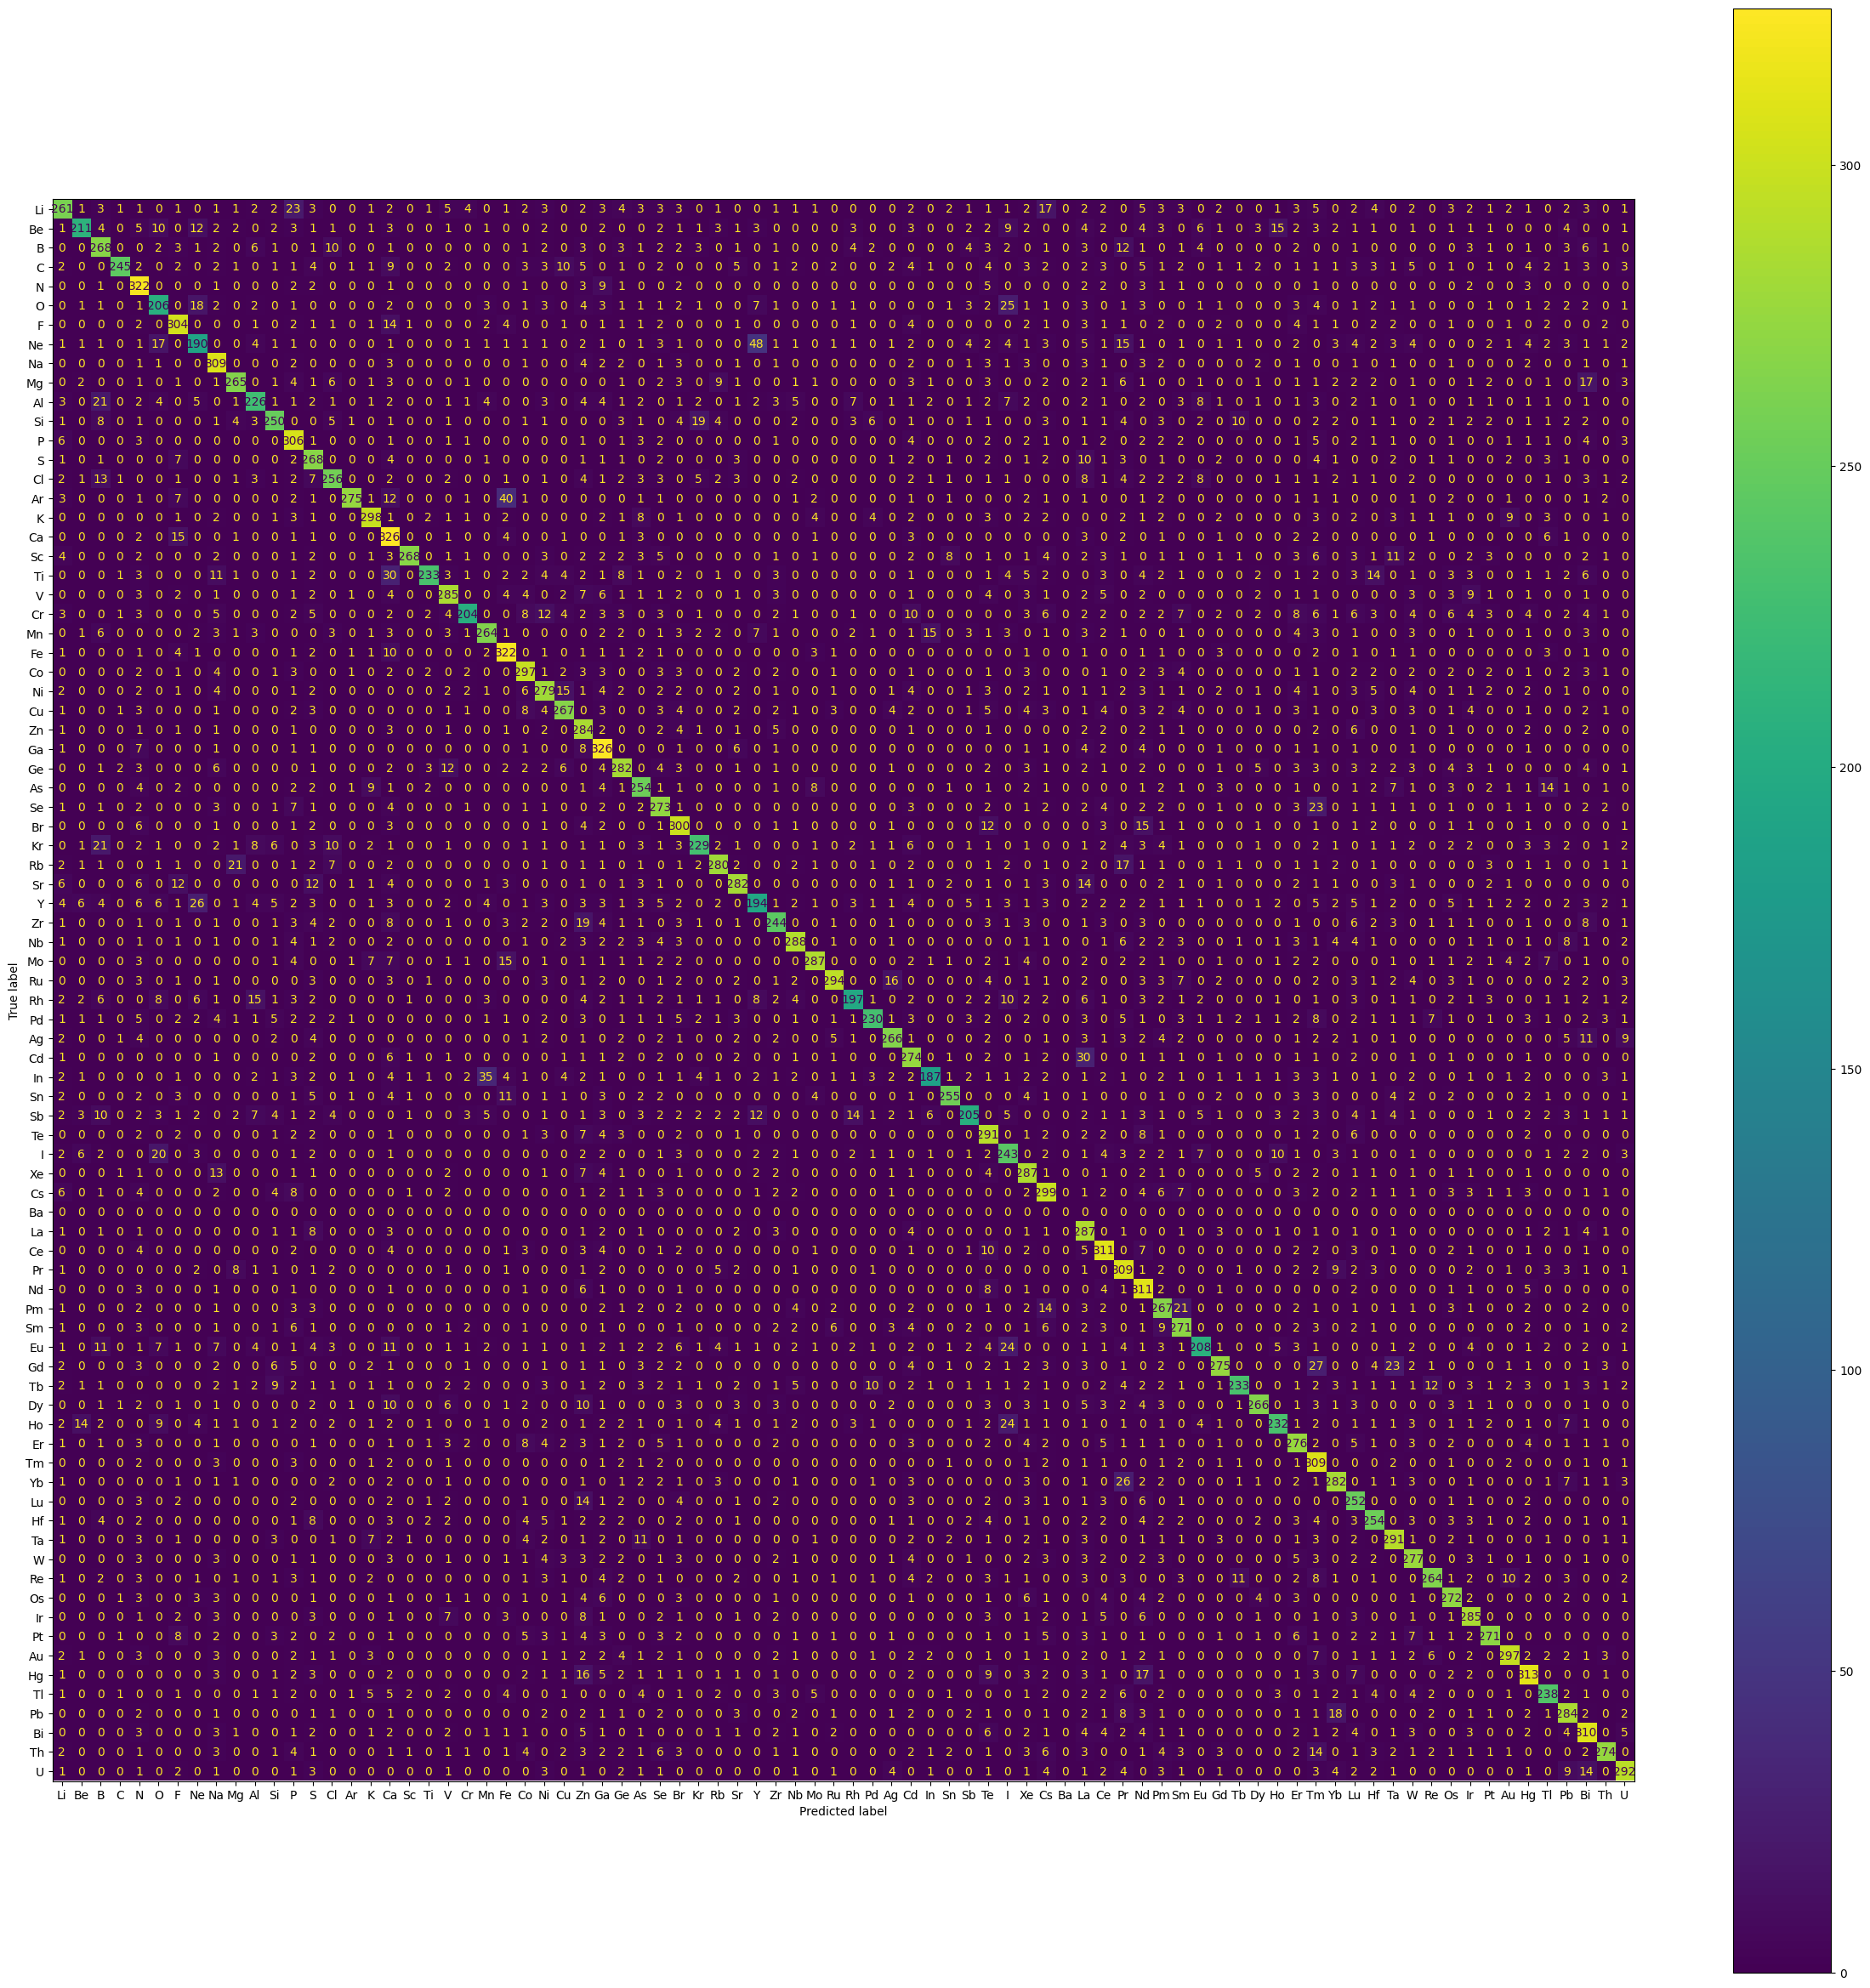
\includegraphics[width=\textwidth]{Figures/CM_CNN_1L.png}
    \centering
    \caption{Confusion Matrix of Test-Data for CNN Top-Layer prediction}
    \label{cm_cnn_1l}
\end{figure}
\end{center}


% from https://www.zhaw.ch/en/lsfm/study/studiweb/master-ls/masters-thesis/
%% !TEX root = ../main.tex

%----------------------------------------------------------------------------------------
% APPENDIX TEMPLATE
%----------------------------------------------------------------------------------------

\chapter{Confusion matrices} % Main appendix title

\label{AppendixB} % Change X to a consecutive letter; for referencing this appendix elsewhere, use \ref{AppendixX}


\begin{center}
\begin{figure}
        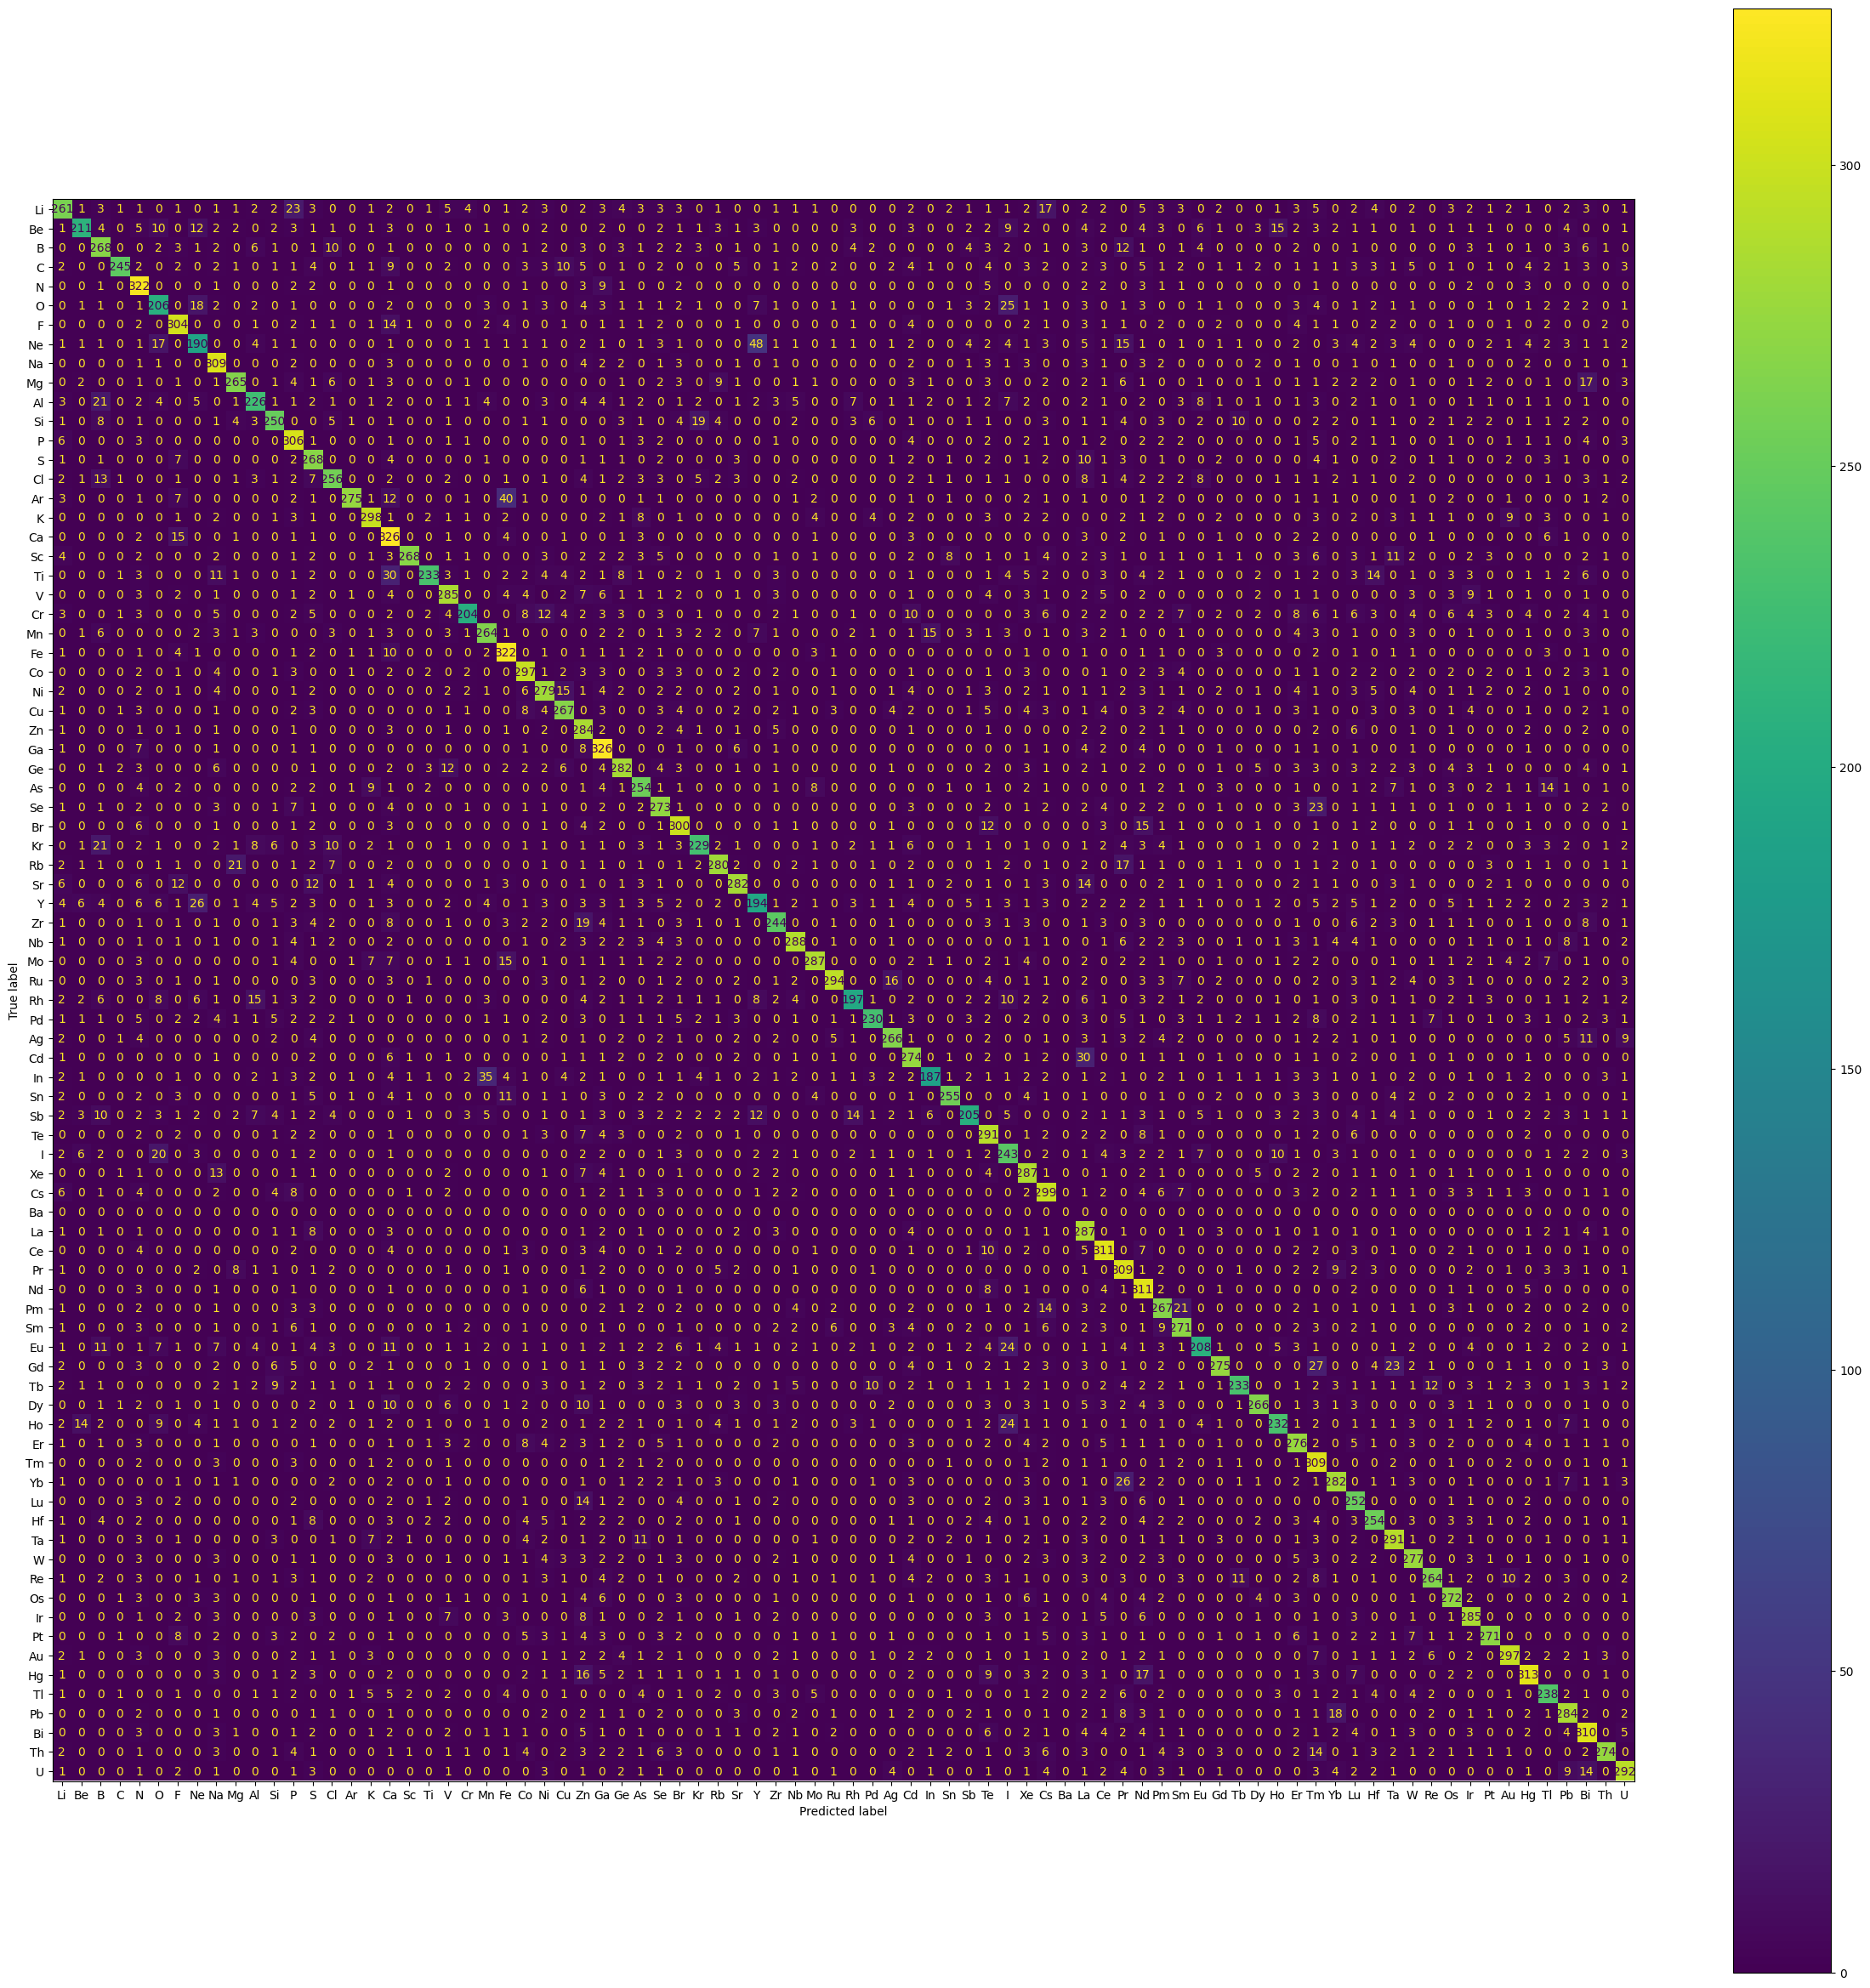
\includegraphics[width=\textwidth]{Figures/CM_CNN_1L.png}
    \centering
    \caption{Confusion Matrix of Test-Data for CNN Top-Layer prediction}
    \label{cm_cnn_1l}
\end{figure}
\end{center}


%\include{Appendices/AppendixC}
% !TEX root = ../main.tex

%----------------------------------------------------------------------------------------
% APPENDIX: DECLARATION OF ORIGINALITY
%----------------------------------------------------------------------------------------

% Include the official "Plagiatserklärung" as a PDF

% Ensure that a TOC entry is create while suppressing the chapter header
\cleardoublepage
\phantomsection
\addtocounter{chapter}{1}
\addcontentsline{toc}{chapter}{\protect\numberline{\thechapter} Declaration of Originality}
% The above replaces this command (which creates a chapter header).
%\chapter{Declaration of Originality} % Main appendix title
\label{DeclarationOfOriginalityZHAW}

% Include a PDF (full page)

\includepdf[pages=-]{Appendices/Declaration of originality Master's Thesis.pdf}
 


%----------------------------------------------------------------------------------------
% BIBLIOGRAPHY
%----------------------------------------------------------------------------------------
\printbibliography[heading=bibintoc]

%----------------------------------------------------------------------------------------

\end{document}  
